\documentclass[11pt,oneside]{article}

\usepackage[T1]{fontenc}
\usepackage[utf8]{inputenc}
\usepackage[english]{babel}
\usepackage{mathtools}
\usepackage{amsthm}
\usepackage{amssymb}
\usepackage{newtxtext,newtxmath}
\usepackage{mathrsfs}
\usepackage{microtype}
\usepackage[a4paper,margin=27mm,headheight=15pt]{geometry}
\usepackage{booktabs,longtable,array,tabularx}
\usepackage{enumitem}
\usepackage{xcolor}
\usepackage[most]{tcolorbox}
\usepackage{listings}
\usepackage{tikz}
\usetikzlibrary{arrows.meta,positioning,calc,matrix}
\usepackage{fancyhdr}
\usepackage{titlesec}
\usepackage{caption}
\usepackage{hyperref}
\usepackage[nameinlink,capitalise,noabbrev]{cleveref}
% Canonical mathematical notation for active FabiusFunction LaTeX documents.
%
% This file is intentionally a plain TeX input rather than a LaTeX package.
% Every standalone document loads it by an explicit path relative to that
% document's directory; included fragments inherit the definitions from their
% root document.  Keep this file independent of document layout and metadata.
%
% Contract:
%   * one command has one mathematical meaning throughout the active corpus;
%   * names encode semantic roles rather than a document-local choice of letter;
%   * visually similar but differently normalized objects have different print;
%   * every command below is defined normatively in the notation catalogue.
%
% The active corpus excludes docs/archive/.  Historical sources may retain
% their original notation only inside an explicitly labelled quotation.

\makeatletter
\@ifundefined{mathbb}{%
  \PackageError{fabius-notation}{The amssymb package must be loaded first}%
    {Load amsmath and amssymb before inputting fabius-notation.tex.}%
}{}
\@ifundefined{operatorname}{%
  \PackageError{fabius-notation}{The amsmath package must be loaded first}%
    {Load amsmath before inputting fabius-notation.tex.}%
}{}
\makeatother

% Version stamp used by the catalogue and by static audits.
\newcommand{\FabiusNotationVersion}{2026-08-31}

% Number systems.  NaturalNumbers is explicitly the nonnegative convention.
\newcommand{\NaturalNumbers}{\mathbb{N}_{0}}
\newcommand{\PositiveIntegers}{\mathbb{N}_{>0}}
\newcommand{\IntegerNumbers}{\mathbb{Z}}
\newcommand{\RationalNumbers}{\mathbb{Q}}
\newcommand{\RealNumbers}{\mathbb{R}}
\newcommand{\ComplexNumbers}{\mathbb{C}}
\newcommand{\ExtendedRealNumbers}{\overline{\mathbb{R}}}

% The three principal Fabius--Rvachev functions.  Subscripts are deliberate:
% a bare F and a calligraphic F have several unrelated uses in the corpus.
\newcommand{\FabiusBounded}{F_{\mathrm{bd}}}
\newcommand{\FabiusGlobal}{F_{\mathrm{gl}}}
\newcommand{\FabiusQuantile}{Q_{F}}
\newcommand{\FabiusClampedQuantile}{Q_{F,\mathrm{cl}}}
\newcommand{\RvachevUp}{\operatorname{up}}

% Constants, elementary operators, and delimiters.
\newcommand{\EulerE}{\mathrm{e}}
\newcommand{\ImaginaryUnit}{\mathrm{i}}
\newcommand{\Differential}{\mathop{}\!\mathrm{d}}
\newcommand{\AbsoluteValue}[1]{\left\lvert #1\right\rvert}
\newcommand{\Norm}[1]{\left\lVert #1\right\rVert}
\newcommand{\Floor}[1]{\left\lfloor #1\right\rfloor}
\newcommand{\Ceiling}[1]{\left\lceil #1\right\rceil}
\newcommand{\FractionalPart}[1]{\left\{#1\right\}}
\newcommand{\PositivePart}[1]{\left(#1\right)_{+}}
\newcommand{\IndicatorOf}[1]{\mathbf{1}_{#1}}
\newcommand{\SetOf}[1]{\left\{#1\right\}}
\newcommand{\InnerProduct}[1]{\left\langle #1\right\rangle}
\newcommand{\CardinalityOf}[1]{\left\lvert #1\right\rvert}
\newcommand{\DefinitionEquals}{\mathrel{\coloneqq}}
\newcommand{\Sign}{\operatorname{sgn}}
\newcommand{\IdentityOperator}{\operatorname{id}}
\newcommand{\SpanOperator}{\operatorname{span}}
\newcommand{\TraceOperator}{\operatorname{tr}}
\newcommand{\RankOperator}{\operatorname{rank}}
\newcommand{\DiagonalOperator}{\operatorname{diag}}
\newcommand{\ResidueOperator}{\operatorname*{Res}}
\newcommand{\LeastCommonMultiple}{\operatorname{lcm}}
\newcommand{\OrderOperator}{\operatorname{ord}}
\newcommand{\PrincipalLogarithm}{\operatorname{Log}}
\newcommand{\FallingFactorial}[2]{\left(#1\right)^{\underline{#2}}}
\newcommand{\RisingFactorial}[2]{\left(#1\right)^{\overline{#2}}}

% Support, topology, convolution, and metric notation.
\newcommand{\SupportOperator}{\operatorname{supp}}
\newcommand{\SupportOf}[1]{\SupportOperator\!\left(#1\right)}
\newcommand{\TopologicalSupportOf}[1]{\operatorname{tsupp}\!\left(#1\right)}
\newcommand{\Convolution}{\mathbin{*}}
\newcommand{\MetricDistance}{\operatorname{dist}}
\newcommand{\TotalVariationDistance}{d_{\mathrm{TV}}}

% Probability.  Equality and convergence in law are not metric distance.
\newcommand{\Probability}{\mathbb{P}}
\newcommand{\Expectation}{\mathbb{E}}
\newcommand{\Variance}{\operatorname{Var}}
\newcommand{\Covariance}{\operatorname{Cov}}
\newcommand{\LawOperator}{\operatorname{Law}}
\newcommand{\LawOf}[1]{\LawOperator\!\left(#1\right)}
\newcommand{\EqualInLaw}{\mathrel{\overset{\mathrm{law}}{=}}}
\newcommand{\ConvergesInLaw}{\mathrel{\xrightarrow{\mathrm{law}}}}

% Fourier and integral transforms.  The printed labels expose normalization.
% FourierTwoPi uses exp(-2*pi*i*x*xi); FourierAngular uses exp(-i*x*omega).
\newcommand{\FourierTwoPi}[1]{\widehat{#1}_{\,2\pi}}
\newcommand{\FourierAngular}[1]{\widehat{#1}_{\,\mathrm{ang}}}
\newcommand{\LaplaceTransformSymbol}{\mathcal{L}}
\newcommand{\MellinTransformSymbol}{\mathcal{M}}
\newcommand{\LaplaceTransformOf}[1]{\LaplaceTransformSymbol\!\left[#1\right]}
\newcommand{\MellinTransformOf}[1]{\MellinTransformSymbol\!\left[#1\right]}
\newcommand{\MomentGeneratingFunction}[1]{M_{#1}}
\newcommand{\CharacteristicFunction}[1]{\varphi_{#1}}

% The two standard sinc functions must never share one symbol.
\newcommand{\SincRad}{\operatorname{sinc}_{\mathrm{rad}}}
\newcommand{\SincPi}{\operatorname{sinc}_{\pi}}

% Binary arithmetic and Thue--Morse notation.
\newcommand{\BinaryDigitSum}{\operatorname{wt}_{2}}
\newcommand{\ThueMorseSignSymbol}{\varepsilon}
\newcommand{\ThueMorseSign}[1]{\varepsilon_{#1}}
\newcommand{\PadicValuation}[1]{\nu_{#1}}
\newcommand{\TwoAdicValuation}{\nu_{2}}

% q-series notation.  Every base is an explicit argument.
\newcommand{\QPochhammer}[3]{\left(#1;#2\right)_{#3}}
\newcommand{\GaussianBinomial}[3]{%
  \genfrac{[}{]}{0pt}{}{#1}{#2}_{#3}%
}
\newcommand{\QInteger}[2]{\left[#1\right]_{#2}}

% Named special functions.
\newcommand{\Polylogarithm}{\operatorname{Li}}
\newcommand{\LambertW}{W}
\newcommand{\GammaFunction}{\Gamma}
\newcommand{\RiemannZeta}{\zeta}

% Asymptotics.  BigO and LittleO are operator tokens for existing formula
% grammar; prefer the At forms so that the limiting regime is printed.
\newcommand{\BigO}{\mathcal{O}}
\newcommand{\LittleO}{o}
\newcommand{\BigOAt}[2]{\mathcal{O}_{#2}\!\left(#1\right)}
\newcommand{\LittleOAt}[2]{o_{#2}\!\left(#1\right)}


\definecolor{ink}{HTML}{1D2733}
\definecolor{accent}{HTML}{4A5D23}
\definecolor{accenttwo}{HTML}{7A5C38}
\definecolor{shade}{HTML}{F3F1E7}
\definecolor{coolshade}{HTML}{EEF2F1}
\definecolor{warmshade}{HTML}{F7EEE9}
\definecolor{codebg}{HTML}{F4F4F2}
\definecolor{rulegray}{HTML}{B8B8AE}

\hypersetup{
  colorlinks=true,
  linkcolor=accent,
  citecolor=accenttwo,
  urlcolor=accenttwo,
  pdftitle={Polynomial-Logarithmic Transseries},
  pdfauthor={OpenAI},
  pdfsubject={Multiplication, division, composition, series reversal, and Lambert W},
  pdfkeywords={transseries, logarithmic asymptotics, Lambert W, series reversion, composition}
}

\pagestyle{fancy}
\fancyhf{}
\fancyhead[L]{\small\itshape Polynomial-Logarithmic Transseries}
\fancyhead[R]{\small\thepage}
\renewcommand{\headrulewidth}{0.4pt}
\fancypagestyle{plain}{\fancyhf{}\fancyfoot[C]{\thepage}\renewcommand{\headrulewidth}{0pt}}

\titleformat{\section}{\Large\bfseries\color{ink}}{\thesection}{0.75em}{}
\titleformat{\subsection}{\large\bfseries\color{ink}}{\thesubsection}{0.7em}{}
\titleformat{\subsubsection}{\normalsize\bfseries\color{ink}}{\thesubsubsection}{0.6em}{}
\setlist{itemsep=0.3em,topsep=0.5em}
\setlength{\parindent}{1.3em}
\setlength{\parskip}{0.18em}
\allowdisplaybreaks
\numberwithin{equation}{section}

\newtheorem{theorem}{Theorem}[section]
\newtheorem{proposition}[theorem]{Proposition}
\newtheorem{lemma}[theorem]{Lemma}
\newtheorem{corollary}[theorem]{Corollary}
\newtheorem{criterion}[theorem]{Criterion}
\theoremstyle{definition}
\newtheorem{definition}[theorem]{Definition}
\newtheorem{example}[theorem]{Example}
\newtheorem{algorithm}[theorem]{Algorithm}
\newtheorem{remark}[theorem]{Remark}
\newtheorem{warning}[theorem]{Warning}

\newtcolorbox{summarybox}[1][]{enhanced,breakable,colback=shade,colframe=accent,
  boxrule=0.7pt,arc=1.4mm,left=2.5mm,right=2.5mm,top=2mm,bottom=2mm,
  fonttitle=\bfseries,title={#1}}
\newtcolorbox{warningbox}[1][]{enhanced,breakable,colback=warmshade,colframe=accenttwo,
  boxrule=0.7pt,arc=1.4mm,left=2.5mm,right=2.5mm,top=2mm,bottom=2mm,
  fonttitle=\bfseries,title={#1}}
\newtcolorbox{examplebox}[1][]{enhanced,breakable,colback=coolshade,colframe=rulegray,
  boxrule=0.6pt,arc=1.2mm,left=2.5mm,right=2.5mm,top=2mm,bottom=2mm,
  fonttitle=\bfseries,title={#1}}

\lstdefinestyle{pseudocode}{
  basicstyle=\ttfamily\small,
  backgroundcolor=\color{codebg},
  frame=single,
  rulecolor=\color{rulegray},
  columns=fullflexible,
  keepspaces=true,
  showstringspaces=false,
  breaklines=true,
  xleftmargin=0.8em,
  framexleftmargin=0.4em,
  aboveskip=0.8em,
  belowskip=0.8em
}

\newcommand{\K}{\mathbb{K}}
\newcommand{\PL}{\PolynomialLogLaurentRing{\K}}
\newcommand{\RL}{\RationalLogLaurentField{\K}}
\newcommand{\HL}{\IteratedLaurentLogField{\K}}
\newcommand{\Gnear}{\NearIdentityPolynomialLogGroup{\K}}
\newcommand{\ordx}{\nu_t}
\newcommand{\lc}{\operatorname{lc}}
\newcommand{\LeadingMonomialOf}[1]{\operatorname{lm}\!\left(#1\right)}
\newcommand{\dlog}{\partial_{\ell}}
\newcommand{\rev}{\langle-1\rangle_{\circ}}
\newcommand{\as}{\sim}
\newcommand{\TransseriesCoefficientOf}[2]{\left[#1\right]\,#2}
\newcommand{\TransseriesTruncateBelow}[2]{%
  \operatorname{Trunc}_{<#2}\!\left(#1\right)%
}
\DeclareMathOperator{\degell}{deg_{\ell}}

\begin{document}
\pagenumbering{roman}
\hypersetup{pageanchor=false}

\begin{titlepage}
\centering
\vspace*{2.5cm}
{\color{accent}\rule{0.86\textwidth}{1.2pt}}\\[1.2cm]
{\Huge\bfseries\color{ink} Polynomial-Logarithmic Transseries\par}
\vspace{0.45cm}
{\LARGE Algebra, Composition, Reversion, and the Lambert \(\LambertW\) Function\par}
\vspace{1.2cm}
{\large A self-contained computational and asymptotic treatment\par}
\vfill
\begin{minipage}{0.82\textwidth}
\small
\textbf{Scope.}  We study expansions of the form
\[
  \sum_{n\ge n_0} p_n(\log x)x^{-n},\qquad p_n\in\K[X],
\]
with special attention to the four operations that most often cause mistakes:
multiplication, division, composition, and compositional inversion.  The central
running example is the large-argument expansion of the Lambert \(\LambertW\) function.
The treatment distinguishes formal identities, closure properties, coefficient
algorithms, and analytic asymptotic meaning.
\end{minipage}
\vfill
{\large August 2026\par}
{\color{accent}\rule{0.86\textwidth}{1.2pt}}
\end{titlepage}
\hypersetup{pageanchor=true}
\setcounter{page}{1}

\begin{abstract}
Polynomial-logarithmic transseries are Laurent series in \(x^{-1}\) whose
coefficients are polynomials in \(\ell=\log x\).  They form one of the smallest
useful fragments of the logarithmic-exponential transseries field: small enough
for exact coefficient arithmetic, yet rich enough to express the standard
large-argument expansions of Lambert \(\LambertW\), Wright's omega function, inverse
logarithmic perturbations, and many solutions obtained from implicit equations.

This article develops the fragment as a complete filtered algebraic calculus.
We define its rank-two monomial order and truncation topology; prove convolution,
unit, differentiation, antidifferentiation, admissible-composition, and reversion
theorems; derive explicit coefficient recurrences for products, quotients,
near-identity compositions, and inverse series; and compare fixed-point,
triangular, Newton, and Lagrange--B\"urmann inversion algorithms.  Particular
care is given to operations that leave the polynomial-logarithmic ring.  This
leads naturally to rational-log, Laurent-log, Puiseux-log, and iterated-log
enlargements.

For Lambert \(\LambertW\), the article derives the complete expansion in Lambert
polynomials, proves their differential-operator, integral-recursion, generating-
function, and Stirling-number descriptions, treats complex branches and the real
branch \(\LambertW_{-1}\), and gives numerical and implementation guidance.  Throughout,
``formal'', ``asymptotic'', and ``convergent'' are kept logically separate.
\end{abstract}

\begin{center}
\begin{minipage}{0.92\textwidth}
\small
\textbf{Source note.}  The supplied source bundle contains, among other material,
G.~A. Edgar's expositions of Hahn-series transseries and composition, papers on
transseries and surreal/Hardy-field viewpoints, and several broad tutorials.  The
present article uses those materials as background but deliberately specializes
to the rank-two polynomial-logarithmic class and develops coefficient-level
algorithms not isolated in the broader surveys.  Additional primary references
include the NIST Digital Library of Mathematical Functions, Corless et al. on
Lambert \(\LambertW\), Cohen on Lambert polynomials, Gessel on formal Lagrange inversion,
and van der Hoeven's monograph on transseries.
\end{minipage}
\end{center}

\clearpage
\tableofcontents
\clearpage
\pagenumbering{arabic}

\section{Orientation: why this small transseries class matters}

\subsection{The characteristic shape}

Let \(x\to+\infty\), put
\[
  t=x^{-1},\qquad \ell=\log x,
\]
and consider a formal expression
\begin{equation}\label{eq:pl-shape}
  F(x)=\sum_{n\ge n_0}p_n(\ell)t^n
      =\sum_{n\ge n_0}p_n(\log x)x^{-n},
  \qquad p_n\in\K[X].
\end{equation}
Here \(n_0\in\IntegerNumbers\), so finitely many positive powers of \(x\) are permitted.
At each fixed inverse-power level \(x^{-n}\), only a finite polynomial in
\(\log x\) is allowed.  We call \eqref{eq:pl-shape} a
\emph{polynomial-logarithmic transseries}, abbreviated PL transseries.

The prototype is obtained by inverting
\[
  y+\log y=x.
\]
The inverse is the Wright omega function \(\WrightOmega(x)=\LambertW(\EulerE^x)\), and its expansion
begins
\begin{equation}\label{eq:omega-preview}
\begin{split}
  \WrightOmega(x)={}&x-\ell+\frac{\ell}{x}
  +\frac{\ell^2/2-\ell}{x^2}
  +\frac{\ell^3/3-3\ell^2/2+\ell}{x^3}\\
  &+\frac{\ell^4/4-11\ell^3/6+3\ell^2-\ell}{x^4}+\cdots.
\end{split}
\end{equation}
Every coefficient is a polynomial in \(\ell\).  For \(\LambertW(z)\), take
\(x=\PrincipalLogarithm z\) and \(\ell=\PrincipalLogarithm\PrincipalLogarithm z\), with branch choices recorded explicitly.

PL transseries occupy a useful middle ground.
\begin{itemize}
\item They are more expressive than ordinary Laurent series because logarithms
  are unavoidable under many asymptotic inversions.
\item They are far simpler than unrestricted logarithmic-exponential transseries:
  a truncated PL series can be represented by a finite array of ordinary
  polynomials.
\item Multiplication, differentiation, integration, many divisions, many
  compositions, and all near-identity reversions reduce to exact finite
  calculations at every requested order.
\item Their failure modes are transparent.  For example, \(1/\ell\),
  \(\log\ell\), and \(x^{1/2}\) each indicate a specific minimal enlargement.
\end{itemize}

\subsection{Four meanings that must not be conflated}

The same displayed series can be read in several ways.

\begin{definition}[Formal PL series]
A formal PL series is an element of the algebra defined in
\cref{sec:formal-ring}.  Equality means equality of every coefficient polynomial;
no value of \(x\) is substituted.
\end{definition}

\begin{definition}[Poincar\'e PL expansion]
A function \(f\) has the expansion
\[
  f(x)\as\sum_{n\ge n_0}p_n(\log x)x^{-n}
\]
as \(x\to+\infty\) if, after including all terms through inverse-power level
\(N-1\), the remainder is \(o(x^{-N+\varepsilon})\) for every fixed
\(\varepsilon>0\); equivalently, it is smaller than every monomial at all
retained levels and larger only at omitted levels.  A sharper and usually more
convenient formulation is given in \cref{sec:analytic-meaning}.
\end{definition}

A formal series can also converge numerically for sufficiently large \(x\), or
be summable by an external analytic procedure.  Neither follows merely from
formal existence.  Conversely, a convergent expansion is automatically formal
when its coefficients are compared algebraically.  Lambert \(\LambertW\) is unusually
pleasant: its canonical inverse-logarithmic series is asymptotic and, in a
sufficiently large domain, genuinely convergent.

\subsection{What the article proves}

The main algebraic conclusions may be summarized in advance.

\begin{summarybox}[Closure map]
Let \(\PL=\K[\ell]((x^{-1}))\).
\begin{enumerate}[label=\textup{(\roman*)}]
\item \(\PL\) is a differential algebra and is closed under indefinite
  integration up to an additive constant.
\item It is closed under multiplication, with ordinary Cauchy convolution in
  the \(x^{-1}\)-index.
\item It is not a field.  A series is a unit precisely when its leading
  coefficient polynomial is a nonzero constant.  General division belongs to
  \(\K(\ell)((x^{-1}))\), and its large-\(\ell\) expansion belongs to
  \(\K((\ell^{-1}))((x^{-1}))\).
\item If the inner argument is
  \(G=cx^q(1+U)\), where \(q\in\PositiveIntegers\), \(c\ne0\), and
  \(U\in x^{-1}\K[\ell][[x^{-1}]]\), then \(F\circ G\in\PL\) after choosing
  \(\log c\).  For rational \(q\), one naturally obtains a Puiseux-log series.
\item The near-identity class
  \(\Gnear=\{x+A:A\in\K[\ell][[x^{-1}]]\}\) is a group under composition.
  Its inverse is computable by a contracting fixed point, triangular
  coefficient matching, Newton iteration, or a Lagrange--B\"urmann formula.
\end{enumerate}
\end{summarybox}

\section{The formal polynomial-logarithmic ring}\label{sec:formal-ring}

\subsection{Coefficient field and variables}

Throughout most of the article, \(\K\) is a field of characteristic zero.  For
real asymptotics one can take \(\K=\RealNumbers\); for branch-sensitive analytic work,
\(\K=\ComplexNumbers\); and for exact symbolic computation, \(\K=\RationalNumbers\) or a finite algebraic
extension is often ideal.  The symbols \(x\), \(t=x^{-1}\), and
\(\ell=\log x\) are formal, but the derivation is chosen to reproduce their
analytic relation:
\begin{equation}\label{eq:basic-derivation}
  \frac{\Differential x}{\Differential x}=1,
  \qquad \frac{\Differential t}{\Differential x}=-t^2,
  \qquad \frac{\Differential\ell}{\Differential x}=t.
\end{equation}

\begin{definition}[PL Laurent ring]
The polynomial-logarithmic Laurent ring is
\begin{equation}\label{eq:PL-ring}
  \PL=\K[\ell]((t))
  =\left\{\sum_{n\ge n_0}p_n(\ell)t^n:
      n_0\in\IntegerNumbers,\ p_n\in\K[\ell]\right\}.
\end{equation}
Its power-series subring is
\[
  {\PL}_{\ge0}=\K[\ell][[t]],
\]
and its strictly small ideal is
\[
  \mathfrak m=t\K[\ell][[t]].
\]
\end{definition}

The notation is an \emph{iterated} Laurent-series notation: first form the
polynomial coefficient ring \(\K[\ell]\), then form Laurent series in \(t\).
This choice records that inverse powers of \(x\) are the primary asymptotic
levels and powers of \(\log x\) refine each level.

\subsection{Rank-two monomial order}

The monomials are
\[
  t^n\ell^j=x^{-n}(\log x)^j,
  \qquad n\in\IntegerNumbers,\quad j\in\NaturalNumbers.
\]
For positive real \(x\to\infty\), define dominance by
\begin{equation}\label{eq:monomial-order}
  t^n\ell^j\succ t^m\ell^k
  \quad\Longleftrightarrow\quad
  n<m\quad\text{or}\quad(n=m\ \text{and}\ j>k).
\end{equation}
Thus every power of \(x\) dominates every power of \(\log x\):
\[
  x\succ \ell^{1000}\succ1\succ \ell^{-1000}\succ x^{-1}.
\]
Within \(\PL\), negative powers of \(\ell\) are absent, but they will appear in
the field extension \(\HL\) below.

It is often convenient to encode \eqref{eq:monomial-order} by the rank-two
valuation
\begin{equation}\label{eq:valuation-pair}
  v(t^n\ell^j)=(n,-j)\in\IntegerNumbers\times\IntegerNumbers
\end{equation}
with lexicographic order.  A nonzero \(F\in\PL\) has a least valuation because
its \(t\)-exponents are bounded below and the polynomial at the first nonzero
level has finite degree.

\begin{definition}[Leading data]
For nonzero
\(F=\sum_{n\ge n_0}p_n(\ell)t^n\), let
\[
  \ordx F=\min\{n:p_n\ne0\},\qquad
  d(F)=\degell p_{\ordx F}.
\]
If \(a\ell^{d(F)}\) is the leading term of
\(p_{\ordx F}\), then
\[
  \LeadingMonomialOf{F}=t^{\ordx F}\ell^{d(F)},\qquad
  \lc(F)=a.
\]
\end{definition}

The pair \((\ordx F,-d(F))\) is the valuation of \(F\).  Notice that
\(\ordx\) alone is only a coarse valuation: two terms at the same inverse-power
level are distinguished by their log degree.

\subsection{Why all coefficient sums are finite}

The support of \(F\) is
\[
  \CoefficientSupportOf{F}=\{(n,j):\TransseriesCoefficientOf{t^n\ell^j}{F}\ne0\}.
\]
For every fixed \(n\), its fiber in \(j\) is finite, and the set of occurring
\(n\)'s is bounded below.  Consequently every nonempty subset of \(\CoefficientSupportOf{F}\)
has a dominant monomial.  This is the elementary rank-two instance of the
well-based support condition used for Hahn series and general transseries
\cite{EdgarBeginners,Hahn1907}.

For multiplication, a fixed pair \((r,k)\) can arise only from
\(n+m=r\), and there are finitely many such pairs once lower bounds on \(n\) and
\(m\) are fixed.  At each such pair, polynomial multiplication supplies only
finitely many log-degree contributions.  This local finiteness is the basic
reason that all operations below can be performed to finite order.

\subsection{Truncation and completeness}

For \(N\in\IntegerNumbers\), define the inverse-power truncation
\begin{equation}\label{eq:truncation}
  \TransseriesTruncateBelow{F}{N}=\sum_{n<N}p_n(\ell)t^n,
  \qquad F=G+\FormalBigOAt{t^N}{t}
  \Longleftrightarrow F-G\in t^N\K[\ell][[t]].
\end{equation}
A computation ``through order \(x^{-N+1}\)'' means equality after applying
\(\TransseriesTruncateBelow{\,cdot\,}{N}\).
This convention retains \emph{all} powers of \(\ell\) at each retained
\(t\)-level.  It avoids the common ambiguity of a total-degree cutoff in two
variables, which generally does not respect asymptotic dominance.

The metric
\[
  d(F,G)=2^{-\ordx(F-G)}
\]
(on differences with nonnegative \(t\)-order, with the usual convention for
zero) defines the \(t\)-adic topology.  A sequence converges exactly when every
coefficient polynomial eventually stabilizes.  The ring
\(\K[\ell][[t]]\) is complete in this topology.  This elementary completeness
supports geometric series, fixed-point iteration, and Newton reversion.

\begin{remark}[Log-degree truncation is a separate approximation]
A computer implementation may also cap polynomial degree in \(\ell\), but that
is not part of the intrinsic \(t\)-adic topology.  Unless a theorem supplies a
degree bound, silently dropping high log powers can corrupt coefficients at an
already retained inverse-power level.
\end{remark}

\subsection{Degree profiles}

For \(F=\sum p_n(\ell)t^n\), define
\[
  d_F(n)=\begin{cases}\degell p_n,&p_n\ne0,\\-\infty,&p_n=0.\end{cases}
\]
The sequence \(d_F(n)\) is the \emph{log-degree profile}.  In many inverse
problems it is at most affine in \(n\).  For the Lambert expansion,
\(d_F(n)=n\) for \(n\ge1\).  Tracking the profile provides a sharper memory and
complexity estimate than treating every coefficient polynomial as having one
global maximum degree.

\section{Multiplication and division}\label{sec:mul-div}

\subsection{Cauchy convolution over \(\K[\ell]\)}

Write
\[
  F=\sum_{n\ge a}p_n(\ell)t^n,
  \qquad G=\sum_{n\ge b}q_n(\ell)t^n.
\]

\begin{theorem}[Product formula]\label{thm:product}
The product \(FG\in\PL\) is
\begin{equation}\label{eq:product-convolution}
  FG=\sum_{r\ge a+b}r_r(\ell)t^r,
  \qquad
  r_r(\ell)=\sum_{n+m=r}p_n(\ell)q_m(\ell).
\end{equation}
Every coefficient sum in \eqref{eq:product-convolution} is finite.  Moreover,
\[
  \ordx(FG)=\ordx F+\ordx G,
  \qquad d(FG)=d(F)+d(G),
  \qquad \lc(FG)=\lc(F)\lc(G).
\]
\end{theorem}

\begin{proof}
For fixed \(r\), the bounds \(n\ge a\) and \(m\ge b\), together with
\(n+m=r\), imply \(a\le n\le r-b\); hence only finitely many \(n\) occur.
Each summand is a polynomial in \(\ell\), proving closure.  At the first possible
level \(r=a+b\), only \((n,m)=(a,b)\) contributes, so the leading coefficient
polynomial is \(p_aq_b\).  The assertions about order, degree, and leading
scalar follow from the corresponding facts for ordinary polynomial products.
\end{proof}

The degree profile satisfies the max-plus bound
\begin{equation}\label{eq:degree-convolution}
  d_{FG}(r)\le
  \max_{n+m=r}\bigl(d_F(n)+d_G(m)\bigr).
\end{equation}
Equality can fail through cancellation.  If
\(d_F(n)\le\alpha n+\beta\) and
\(d_G(n)\le\alpha n+\gamma\) over the relevant ranges, then
\(d_{FG}(r)\le\alpha r+\beta+\gamma\).  Thus a common affine slope is stable
under multiplication.

\begin{examplebox}[A complete finite convolution]
Let
\[
 F=1+\ell t+(\ell^2+1)t^2,
 \qquad
 G=2-\ell t+3\ell t^2.
\]
Then
\begin{align*}
 FG={}&2+\ell t+(\ell^2+3\ell+2)t^2\\
 &+(-\ell^3+3\ell^2-\ell)t^3
 +(3\ell^3+3\ell)t^4.
\end{align*}
The calculation is ordinary polynomial multiplication nested inside ordinary
Cauchy convolution.
\end{examplebox}

\subsection{Truncated multiplication}

Suppose only \(\TransseriesTruncateBelow{FG}{N}\) is required.  Terms of \(F\) with exponent
\(n\ge N-b\) and terms of \(G\) with exponent \(m\ge N-a\) cannot contribute.
Hence
\begin{equation}\label{eq:truncated-product}
  \TransseriesTruncateBelow{FG}{N}
  =\sum_{r=a+b}^{N-1}
    \left(\sum_{n=\max(a,r-(N_G-1))}^{\min(N_F-1,r-b)}p_nq_{r-n}\right)t^r,
\end{equation}
where \(N_F,N_G\) denote the available cutoffs.  A robust implementation carries
lower exponents explicitly rather than pretending every series starts at zero.

\subsection{Units in the polynomial-logarithmic ring}

The distinction between a nonzero element and a unit is essential.

\begin{theorem}[Unit criterion]\label{thm:unit-criterion}
Let
\[
  G=t^m\bigl(g_0(\ell)+g_1(\ell)t+g_2(\ell)t^2+\cdots\bigr),
  \qquad g_0\ne0.
\]
Then \(G\) is invertible in \(\PL\) if and only if
\(g_0\in\K^\times\), that is, the leading coefficient polynomial is a nonzero
constant.
\end{theorem}

\begin{proof}
If \(g_0=c\in\K^\times\), factor
\[
  G=c t^m(1+U),\qquad U\in t\K[\ell][[t]],
\]
and use the \(t\)-adically convergent geometric series
\begin{equation}\label{eq:geometric-reciprocal}
  G^{-1}=c^{-1}t^{-m}\sum_{r\ge0}(-U)^r.
\end{equation}
At any fixed \(t\)-order only finitely many powers of \(U\) contribute.

Conversely, suppose \(GH=1\) with \(H\in\PL\).  Comparing leading
\(t\)-levels shows that the leading coefficient polynomials of \(G\) and \(H\)
multiply to \(1\) in \(\K[\ell]\).  The only units of a polynomial ring over a
field are nonzero constants, so \(g_0\) must be constant.
\end{proof}

\begin{warningbox}[A frequent category error]
The ring \(\K[\ell]((t))\) is not a field.  For example,
\[
  \ell^{-1}\notin\PL,
  \qquad
  (\ell+t)^{-1}\notin\PL.
\]
Calling every nonzero PL series ``invertible'' silently changes the coefficient
ring.  The appropriate extensions are described in
\cref{subsec:field-extensions}.
\end{warningbox}

\subsection{Reciprocal recurrence}

Let
\[
  G=\sum_{n\ge0}g_n(\ell)t^n,
  \qquad g_0=c\in\K^\times,
  \qquad
  G^{-1}=\sum_{n\ge0}b_n(\ell)t^n.
\]
Comparing coefficients in \(GG^{-1}=1\) gives
\begin{equation}\label{eq:reciprocal-recurrence}
  b_0=c^{-1},
  \qquad
  b_n=-c^{-1}\sum_{k=1}^{n}g_kb_{n-k}
  \quad(n\ge1).
\end{equation}
This recurrence is usually preferable to expanding the geometric series
literally: it computes each new coefficient once and exposes exact polynomial
cancellation.

\begin{example}
For \(G=1+\ell t+t^2\), \eqref{eq:reciprocal-recurrence} yields
\begin{align*}
 G^{-1}={}&1-\ell t+(\ell^2-1)t^2+(-\ell^3+2\ell)t^3\\
 &+(\ell^4-3\ell^2+1)t^4
 +(-\ell^5+4\ell^3-3\ell)t^5+\cdots.
\end{align*}
The coefficient polynomials obey the second-order recurrence
\(b_n=-\ell b_{n-1}-b_{n-2}\).
\end{example}

\subsection{Long division and quotient recurrence}

Suppose
\[
 F=\sum_{n\ge0}f_n t^n,
 \qquad G=\sum_{n\ge0}g_n t^n,
 \qquad g_0=c\in\K^\times,
 \qquad H=F/G=\sum_{n\ge0}h_n t^n.
\]
Then
\begin{equation}\label{eq:quotient-recurrence}
  h_0=c^{-1}f_0,
  \qquad
  h_n=c^{-1}\left(f_n-\sum_{k=1}^{n}g_kh_{n-k}\right).
\end{equation}
The same formula works for Laurent series after first shifting the leading
powers of \(t\).  It is triangular: \(h_n\) depends only on earlier quotient
coefficients.

If \(g_0(\ell)\) is nonconstant, the same recurrence is valid in
\(\K(\ell)\), and it is also an exact divisibility test in \(\K[\ell]\): at every
step the numerator must be divisible by \(g_0\).  A quotient can therefore lie in
\(\PL\) even when \(G\) is not a unit, but this is exceptional and must be
verified coefficient by coefficient.

\subsection{The minimal field extensions}\label{subsec:field-extensions}

Three nested coefficient choices are useful:
\begin{align}
 \PL&=\K[\ell]((t)),\label{eq:ring-hierarchy-a}\\
 \RL&=\K(\ell)((t)),\label{eq:ring-hierarchy-b}\\
 \HL&=\K((\ell^{-1}))((t)).\label{eq:ring-hierarchy-c}
\end{align}
Here \(\RL\) is a field of Laurent series in \(t\) with rational functions of
\(\ell\) as coefficients.  The field \(\HL\) expands each rational-log
coefficient at \(\ell=\infty\), allowing finitely many positive and arbitrarily
many negative powers of \(\ell\).  For example,
\begin{align*}
  \frac{1}{\ell+t}
  &=\frac1\ell\frac{1}{1+t/\ell}
    =\ell^{-1}-t\ell^{-2}+t^2\ell^{-3}-\cdots\in\HL,\\
  \frac{1}{\ell^2+\ell+1}
  &=\ell^{-2}\left(1+\ell^{-1}+\ell^{-2}\right)^{-1}
    \in\K((\ell^{-1})).
\end{align*}

\begin{proposition}[Field property]
Both \(\RL\) and \(\HL\) are fields.  Every nonzero element of \(\PL\) becomes
invertible in \(\RL\), and its large-\(\ell\) reciprocal expansion belongs to
\(\HL\).
\end{proposition}

\begin{proof}
A Laurent-series ring \(E((t))\) over a field \(E\) is a field: factor a nonzero
series as \(t^m a(1+U)\), where \(a\in E^\times\) and \(U\in tE[[t]]\), then use
\eqref{eq:geometric-reciprocal}.  Take \(E=\K(\ell)\) or
\(E=\K((\ell^{-1}))\).  A nonzero polynomial in \(\ell\) is invertible in
\(\K(\ell)\); factoring its leading power of \(\ell\) and geometrically expanding
the lower-degree part gives an element of \(\K((\ell^{-1}))\).
\end{proof}

The order of iteration matters.  The fields
\(\K((\ell^{-1}))((t))\) and \(\K((t))((\ell^{-1}))\) impose different support
conditions, just as iterated Laurent-series fields in ordinary formal-power-
series theory are generally different \cite{GesselLagrange}.  Our choice makes
\(t=x^{-1}\) the primary scale, matching the intended asymptotic hierarchy.

\subsection{Local analytic functional calculus}

Let \(U\in\mathfrak m\), and let
\(\Phi(z)=\sum_{r\ge0}c_r(z-a)^r\) be a formal or convergent power series about
\(a\in\K\).  Then
\begin{equation}\label{eq:local-functional-calculus}
  \Phi(a+U)=\sum_{r\ge0}c_rU^r\in\K[\ell][[t]]
\end{equation}
is well-defined \(t\)-adically.  In particular,
\begin{align}
 (1+U)^\alpha&=\sum_{r\ge0}\binom{\alpha}{r}U^r,\label{eq:binomial-U}\\
 \log(1+U)&=\sum_{r\ge1}\frac{(-1)^{r+1}}{r}U^r,\label{eq:log-U}\\
 \EulerE^U&=\sum_{r\ge0}\frac{U^r}{r!}.\label{eq:exp-U}
\end{align}
These formulas are formal; analytic convergence for a numerical \(x\) is a
separate issue.

The restrictions are important.  If \(P(\ell)\) is a nonlinear polynomial,
then \(\EulerE^{P(\ell)}\) is generally not a PL series: for example,
\(\EulerE^{\ell^2}=x^{\ell}\) introduces a new exponential monomial.  By contrast,
\(\EulerE^{a\ell+b}=\EulerE^b x^a\) remains in a generalized-power extension, and remains in
\(\PL\) when \(a\in\IntegerNumbers\).

\section{Differential and integral calculus}\label{sec:differential}

\subsection{The basic lowering operator on coefficient polynomials}

For a monomial level \(t^n p(\ell)=x^{-n}p(\log x)\), the chain rule gives
\begin{equation}\label{eq:one-derivative}
  \frac{\Differential}{\Differential x}\bigl(t^n p(\ell)\bigr)
  =t^{n+1}(\dlog-n)p(\ell).
\end{equation}
Thus differentiation raises the \(t\)-order by one and applies a first-order
operator to the log polynomial.

\begin{definition}[Shifted logarithmic differential operator]
For \(n\in\IntegerNumbers\) and \(k\in\NaturalNumbers\), set
\begin{equation}\label{eq:Delta-def}
  \Delta_{n,k}
  =\prod_{j=0}^{k-1}(\dlog-n-j),
  \qquad \Delta_{n,0}=1.
\end{equation}
The factors commute because each is a polynomial in \(\dlog\).
\end{definition}

\begin{proposition}[Repeated derivative]\label{prop:repeated-derivative}
For every \(k\ge0\),
\begin{equation}\label{eq:repeated-derivative}
  \frac{\Differential^k}{\Differential x^k}\bigl(t^n p(\ell)\bigr)
  =t^{n+k}\Delta_{n,k}p(\ell).
\end{equation}
Consequently \(\PL\) is closed under differentiation.
\end{proposition}

\begin{proof}
The case \(k=0\) is immediate and the case \(k=1\) is
\eqref{eq:one-derivative}.  If \eqref{eq:repeated-derivative} holds for \(k\),
apply \eqref{eq:one-derivative} at level \(n+k\):
\[
 D\bigl(t^{n+k}\Delta_{n,k}p\bigr)
 =t^{n+k+1}(\dlog-n-k)\Delta_{n,k}p
 =t^{n+k+1}\Delta_{n,k+1}p.
\]
Termwise differentiation is locally finite at every \(t\)-level.
\end{proof}

A useful expanded form follows from the signed Stirling numbers of the first
kind.  Since
\[
  \prod_{j=0}^{k-1}(z-n-j)=(z-n)^{\underline{k}},
\]
\(\Delta_{n,k}\) is a degree-\(k\) polynomial in \(\dlog\).  Because differentiation
of a polynomial is nilpotent, only finitely many terms act nontrivially on any
fixed coefficient.

\subsection{Valuation behavior}

For nonzero \(F\in\PL\), one always has
\[
  \ordx F'\ge\ordx F+1.
\]
Equality can fail.  At level \(n=0\), a constant coefficient differentiates to
zero; more generally, cancellations may annihilate the leading coefficient.
For a leading term \(a t^n\ell^d\):
\begin{itemize}
\item if \(n\ne0\), then \(F'\) has leading term
  \(-na t^{n+1}\ell^d\);
\item if \(n=0\) and \(d>0\), then it has leading term
  \(ad t\ell^{d-1}\);
\item if \(n=d=0\), the leading constant disappears and the next term decides.
\end{itemize}
This distinction is central in the contraction proof for compositional inverses:
if \(A\in\K[\ell][[t]]\), then \(A'\in t\K[\ell][[t]]\).

\subsection{Antidifferentiation stays in the class}

Unlike many restricted asymptotic scales, \(\PL\) is also closed under
indefinite integration.

\begin{theorem}[Termwise antiderivative]\label{thm:antiderivative}
For every \(F\in\PL\), there exists \(G\in\PL\) with \(G'=F\).  It is unique up
to an additive constant in \(\K\).
\end{theorem}

\begin{proof}
It suffices to integrate one term \(t^n p(\ell)=x^{-n}p(\ell)\).
If \(n\ne1\), seek an antiderivative of the form
\(x^{1-n}q(\ell)=t^{n-1}q(\ell)\).  Differentiation gives
\[
  \frac{\Differential}{\Differential x}\bigl(x^{1-n}q(\ell)\bigr)
  =x^{-n}\bigl(q'(\ell)+(1-n)q(\ell)\bigr).
\]
The operator \(\dlog+(1-n)\) is invertible on \(\K[\ell]\) when
\(1-n\ne0\): solve recursively from the highest polynomial degree downward.
If \(n=1\), then
\[
  \int x^{-1}p(\log x)\Differential x=\int p(\ell)\Differential\ell,
\]
which is again a polynomial in \(\ell\) because \(\operatorname{char}\K=0\).
Termwise integration is locally finite, and the only kernel of the derivation in
\(\PL\) is \(\K\).
\end{proof}

For \(n\ne1\), an explicit finite formula is
\begin{equation}\label{eq:antiderivative-explicit}
  (\dlog+1-n)^{-1}p
  =\frac{1}{1-n}\sum_{j=0}^{\deg p}
    \left(-\frac{\dlog}{1-n}\right)^j p.
\end{equation}
The sum terminates because sufficiently many derivatives of \(p\) vanish.

\subsection{Product, quotient, and chain rules}

Because all operations are defined coefficientwise in a complete filtered
algebra, the usual formal rules hold whenever the relevant expression exists:
\begin{align}
 (FG)'&=F'G+FG',\label{eq:product-rule}\\
 (F/G)'&=(F'G-FG')/G^2,\label{eq:quotient-rule}\\
 (F\circ G)'&=(F'\circ G)G'.\label{eq:chain-rule-preview}
\end{align}
For the chain rule, admissibility of the composition must first be established;
this is the subject of \cref{sec:composition}.  The algebraic identities can then
be proved on finite truncations and passed to the \(t\)-adic limit.

\section{Composition}\label{sec:composition}

\subsection{Why substitution needs an admissibility theorem}

For polynomials, substitution is automatic.  For an infinite series it is not.
If one writes
\[
  \left(\sum_n a_nM_n\right)\circ G
  =\sum_n a_n(M_n\circ G),
\]
one must prove that only finitely many summands contribute to each output
monomial.  Otherwise a single coefficient would be an undefined infinite sum in
\(\K\).  General transseries theory formulates this requirement through
summable families and well-based supports \cite{EdgarBeginners,EdgarComposition,
VanDerHoeven2006}.  In the PL setting it reduces to concrete order estimates.

Three examples show why a blanket rule ``replace \(x\) by \(G\)'' is unsafe:
\begin{align*}
  (x^{-1})\circ\ell&=\ell^{-1}\notin\PL,\\
  (\log x)\circ(x\ell)&=\ell+\log\ell\notin\PL,\\
  (x^{-1})\circ x^{1/2}&=x^{-1/2},
\end{align*}
where the last expression lies in a Puiseux extension rather than in \(\PL\).
The substitutions are meaningful in larger transseries fields, but not closed in
the original ring.

\subsection{Composition with a monomial-leading argument}

The largest natural class of inner arguments that preserves integer-power PL
series has a positive integral power of \(x\) as its leading monomial.

\begin{theorem}[Monomial-leading composition]\label{thm:monomial-composition}
Let
\begin{equation}\label{eq:outer-inner-composition}
  F(y)=\sum_{n\ge a}p_n(\log y)y^{-n}\in\PL
\end{equation}
and let
\begin{equation}\label{eq:admissible-G}
  G(x)=c x^q(1+U(x)),
  \qquad c\in\K^\times,\quad q\in\PositiveIntegers,\quad U\in\mathfrak m.
\end{equation}
Choose a value of \(\log c\) if \(\K\subseteq\ComplexNumbers\).  Then
\begin{equation}\label{eq:composition-master}
\boxed{
  (F\circ G)(x)=
  \sum_{n\ge a}
  p_n\!\left(q\ell+\log c+V\right)
  c^{-n}t^{qn}(1+U)^{-n},
  \qquad V=\log(1+U),
}
\end{equation}
is a well-defined element of \(\PL\).
\end{theorem}

\begin{proof}
By \eqref{eq:log-U}, \(V\in\mathfrak m\).  Since \(p_n\) is a polynomial,
\(p_n(q\ell+\log c+V)\) is a finite sum of powers of \(V\), hence belongs to
\(\K[\ell][[t]]\).  The binomial expansion
\[
  (1+U)^{-n}=\sum_{r\ge0}\binom{-n}{r}U^r
\]
is \(t\)-adically well-defined for every integer \(n\).  The \(n\)-th outer
summand begins at \(t^{qn}\), up to the fixed finite set of negative \(n\)'s.
For a requested output exponent \(N\), only \(n\le N/q\) can contribute.  For
each such \(n\), only finitely many powers of \(U\) and \(V\) can contribute
modulo \(t^{N+1}\).  Thus every coefficient is a finite sum of polynomials in
\(\ell\), proving both summability and closure.
\end{proof}

\begin{remark}[Rational and general powers]
If \(q=r/s\in\RationalNumbers_{>0}\), the same proof works after adjoining
\(x^{1/s}\), giving a Puiseux-log series.  For arbitrary real or complex \(q\),
one enters a generalized Hahn-series scale with monomials \(x^{-\gamma}\).
The obstruction is not composition itself; it is the decision to restrict
exponents to integers.
\end{remark}

\begin{corollary}[Scaling and power substitution]
For \(c\ne0\) and \(q\in\PositiveIntegers\),
\begin{equation}\label{eq:scale-composition}
  F(cx^q)=\sum_{n\ge a}c^{-n}x^{-qn}
             p_n(q\ell+\log c).
\end{equation}
In particular, scaling acts on coefficient polynomials by an affine change of
logarithmic variable.
\end{corollary}

\subsection{Near-identity arguments}

The most important special case is
\begin{equation}\label{eq:near-identity-G}
  G(x)=x+H(x)=x\bigl(1+tH(x)\bigr),
  \qquad H\in{\PL}_{\ge0}.
\end{equation}
Since \(tH\in\mathfrak m\), \cref{thm:monomial-composition} applies with
\(q=1\), \(c=1\), and \(U=tH\).  Analytically, \(H=o(x)\), even when
\(H\) is a polynomial in \(\log x\).

\begin{theorem}[Formal Taylor formula]\label{thm:formal-taylor}
For \(F\in\PL\) and \(H\in{\PL}_{\ge0}\),
\begin{equation}\label{eq:formal-taylor}
\boxed{
  F\circ(x+H)=\sum_{k\ge0}\frac{H^k}{k!}D^kF,
  \qquad D=\frac{\Differential}{\Differential x}.
}
\end{equation}
The family on the right is \(t\)-adically summable.  Modulo \(t^N\), only
finitely many \(k\) are needed.
\end{theorem}

\begin{proof}
Introduce an auxiliary central variable \(s\) and form
\(\Phi(s)=F(x+sH)\) using \cref{thm:monomial-composition}.  Differentiation with
respect to \(s\), holding \(x\) and \(H(x)\) fixed, gives
\[
  \frac{\partial^k\Phi}{\partial s^k}(0)=H^kD^kF.
\]
The formal Taylor expansion in \(s\) therefore gives
\(\Phi(s)=\sum_{k\ge0}s^kH^kD^kF/k!\).  Set \(s=1\).  If
\(a=\ordx F\), then \(D^kF\) has \(t\)-order at least \(a+k\), while
\(H^k\) has nonnegative \(t\)-order.  Hence at output order \(N\), only
\(k\le N-a\) can contribute.  This proves summability and justifies setting
\(s=1\).
\end{proof}

The theorem is an exact identity of formal PL series, not merely an asymptotic
Taylor approximation.  Its validity rests on the filtration: successive Taylor
terms become successively smaller in powers of \(t\).

\subsection{An explicit coefficient formula}

Let
\begin{equation}\label{eq:F-H-components}
 F=\sum_{n\ge a}p_n(\ell)t^n,
 \qquad
 H^k=\sum_{m\ge0}h_{k,m}(\ell)t^m,
 \qquad h_{0,0}=1.
\end{equation}
Combining \cref{prop:repeated-derivative,thm:formal-taylor} yields
\begin{equation}\label{eq:composition-coefficient}
\boxed{
  \TransseriesCoefficientOf{t^r}{F\circ(x+H)}
  =\sum_{\substack{n\ge a,\ k\ge0,\ m\ge0\\n+k+m=r}}
    \frac{h_{k,m}(\ell)}{k!}\,\Delta_{n,k}p_n(\ell).
}
\end{equation}
The sum is finite.  Formula \eqref{eq:composition-coefficient} separates the
three pieces of work:
\begin{enumerate}
\item powers \(H^k\), computed by truncated multiplication;
\item shifted differential operators \(\Delta_{n,k}\) on coefficient
  polynomials;
\item a finite index convolution \(n+k+m=r\).
\end{enumerate}
It is particularly convenient when the same inner correction \(H\) is used to
compose many outer series.

\begin{examplebox}[Composition by \(x+\ell\)]
Let
\[
  F(x)=\ell+\ell^2t,
  \qquad G(x)=x+\ell.
\]
Directly,
\[
  \log G=\ell+\log(1+\ell t),
  \qquad G^{-1}=t(1+\ell t)^{-1}.
\]
Either these formulas or \eqref{eq:composition-coefficient} gives
\begin{align*}
 F\circ G={}&\ell+(\ell^2+\ell)t
 +\left(-\ell^3+\frac32\ell^2\right)t^2\\
 &+\left(\ell^4-\frac83\ell^3+\ell^2\right)t^3\\
 &+\left(-\ell^5+\frac{41}{12}\ell^4-2\ell^3\right)t^4
 +\FormalBigOAt{t^5}{t}.
\end{align*}
The increasing log degree is not accidental: every expansion of
\(\log(1+\ell t)\) supplies another factor of \(\ell\).
\end{examplebox}

\subsection{Composition by an affine perturbation}

For \(G=cx+d+\FormalBigOAt{t}{t}\), factor
\[
  G=cx\left(1+\frac{d}{cx}+\FormalBigOAt{t^2}{t}\right).
\]
Then
\begin{align*}
  \log G
  &=\ell+\log c+\frac{d}{c}t-\frac{d^2}{2c^2}t^2+\cdots,\\
  G^{-n}
  &=c^{-n}t^n\left(1+\frac{d}{c}t+\cdots\right)^{-n}.
\end{align*}
The constant shift \(d\) is therefore handled by the same binomial-logarithmic
calculus as any near-identity correction.  There is no need to introduce a
separate theory of ``series at infinity'' beyond the filtered ring already in
use.

\subsection{Associativity and the chain rule}

Composition is associative only when all displayed compositions are admissible.
Within the monomial-leading domain of \cref{thm:monomial-composition}, the
identity
\begin{equation}\label{eq:composition-associativity}
  (F\circ G)\circ H=F\circ(G\circ H)
\end{equation}
holds whenever \(G\circ H\) again has an admissible positive large leading
monomial.  One proof checks the identity first for the generators \(x\),
\(x^{-1}\), and \(\log x\), then extends through addition, multiplication, and
\(t\)-adic limits.  Another truncates all series, where substitution is a finite
algebraic operation, and lets the cutoff increase.

Under the same hypotheses,
\begin{equation}\label{eq:chain-rule}
  D(F\circ G)=(DF\circ G)DG.
\end{equation}
For near-identity \(G=x+H\), it can also be verified by differentiating
\eqref{eq:formal-taylor} and rearranging the locally finite sums.

\subsection{Exactly where closure fails}

The following table is a practical diagnostic.

\begin{center}
\begin{tabularx}{0.95\textwidth}{@{}>{\raggedright\arraybackslash}p{0.22\textwidth}
>{\raggedright\arraybackslash}p{0.29\textwidth}X@{}}
\toprule
Inner leading behavior & Typical new object & Minimal customary enlargement\\
\midrule
\(cx^q\), \(q\in\PositiveIntegers\) & none & \(\PL\)\\
\(cx^{r/s}\) & fractional powers of \(x\) & Puiseux-log series\\
\(c\ell^q\) & negative powers of \(\ell\) from outer reciprocals & Laurent-log field \(\HL\)\\
\(x\ell^a\) inside an outer logarithm & \(\log\ell\) & one additional iterated-log level\\
\(\EulerE^x\) & exponential monomials & logarithmic-exponential transseries\\
inner series near a branch zero & fractional or ramified local powers & local Puiseux/branch expansion\\
\bottomrule
\end{tabularx}
\end{center}

\begin{warning}
An expression can be meaningful while lying outside \(\PL\).  Closure is a
statement about the chosen representation class, not about existence of the
composed analytic function.
\end{warning}

\section{Compositional inversion and series reversal}\label{sec:reversion}

\subsection{The near-identity composition group}

\begin{definition}[Near-identity PL maps]
Let
\begin{equation}\label{eq:near-group}
  \Gnear=\left\{x+A(x):A\in{\PL}_{\ge0}\right\}.
\end{equation}
Every member satisfies \(x+A\as x\) and has formal derivative
\(1+A'=1+\FormalBigOAt{t}{t}\).
\end{definition}

\begin{theorem}[Group theorem]\label{thm:near-group}
The set \(\Gnear\) is a group under composition.  If
\(F=x+A\in\Gnear\), there is a unique
\(G=x+B\in\Gnear\) such that
\begin{equation}\label{eq:two-sided-inverse}
  F\circ G=G\circ F=x.
\end{equation}
\end{theorem}

\begin{proof}
Closure follows from
\[
  (x+A)\circ(x+B)=x+B+A\circ(x+B),
\]
and \cref{thm:formal-taylor} shows that the correction belongs to
\({\PL}_{\ge0}\).  For existence, solve the fixed-point equation
\begin{equation}\label{eq:fixed-point-B}
  B=\Phi(B):=-A\circ(x+B).
\end{equation}
If \(B-C\in t^N{\PL}_{\ge0}\), the formal mean-value/Taylor identity gives
\[
  A\circ(x+B)-A\circ(x+C)
  =(B-C)\int_0^1 A'\circ(x+C+s(B-C))\Differential s.
\]
Since \(A'\in t{\PL}_{\ge0}\), the right side lies in
\(t^{N+1}{\PL}_{\ge0}\).  Thus \(\Phi\) improves the agreement order by at least
one.  Starting with \(B_0=0\), the iterates
\(B_{j+1}=\Phi(B_j)\) form a Cauchy sequence in the complete \(t\)-adic ring and
converge to a unique fixed point \(B\).  The equation
\(B+A\circ(x+B)=0\) gives \(F\circ G=x\).

A right inverse in this class is automatically two-sided.  Indeed, construct a
right inverse \(H\) of \(G\).  Then
\[
  F=F\circ x=F\circ(G\circ H)=(F\circ G)\circ H=x\circ H=H,
\]
so \(G\circ F=G\circ H=x\).  Uniqueness follows from the contraction: two fixed
points agree modulo \(t^N\) for all \(N\).
\end{proof}

This is the PL specialization of the fixed-point mechanism used for
well-based transseries compositional inverses \cite{EdgarComposition}.  Here the
contraction is visible in the elementary fact \(A'=\FormalBigOAt{t}{t}\).

\subsection{Picard iteration}

The proof supplies the first inversion algorithm:
\begin{equation}\label{eq:picard-reversion}
  B_0=0,
  \qquad B_{j+1}=-A\circ(x+B_j).
\end{equation}
After \(j\) iterations, at least the first \(j\) new inverse-power levels have
stabilized (often more, if \(A'\) begins beyond order \(t\)).  This method is
conceptually simple and excellent for proofs, but it repeatedly recomputes lower
coefficients and is not the fastest high-order algorithm.

\subsection{Triangular coefficient correction}

Suppose an approximation \(G_N=x+B_N\) satisfies
\begin{equation}\label{eq:residual-order-N}
  F\circ G_N-x=r_N(\ell)t^N+\FormalBigOAt{t^{N+1}}{t}.
\end{equation}
Because \(F'\circ G_N=1+\FormalBigOAt{t}{t}\), adding
\(-r_Nt^N\) to \(G_N\) removes the residual at level \(N\):
\begin{equation}\label{eq:triangular-update}
  G_{N+1}=G_N-r_N(\ell)t^N
  \quad\Longrightarrow\quad
  F\circ G_{N+1}=x+\FormalBigOAt{t^{N+1}}{t}.
\end{equation}
Thus inverse coefficients can be found one polynomial at a time.  No linear
system larger than a scalar identity is needed because the leading derivative is
one.  For a more general leading slope \(F(x)=ax+o(x)\), the correction is divided
by \(a\).

\subsection{Newton reversion}

The formal Newton step is
\begin{equation}\label{eq:newton-reversion}
\boxed{
  G_{\mathrm{new}}
  =G-\frac{F\circ G-x}{F'\circ G}.
}
\end{equation}
The denominator is a unit because \(F'=1+\FormalBigOAt{t}{t}\).  If
\(F\circ G-x\in t^N{\PL}_{\ge0}\), Taylor expansion around \(G\) shows that the
new residual is in \(t^{2N+1}{\PL}_{\ge0}\) (the exact exponent can improve with
additional valuation information).  Hence a precision-doubling implementation
uses truncation cutoffs
\(1,2,4,8,\ldots\), recomputing products, composition, and a reciprocal only at
the newly required precision.

\begin{proof}[Residual estimate]
Let \(R=F\circ G-x\) and \(C=-R/(F'\circ G)\).  Since \(C=\FormalBigOAt{t^N}{t}\),
\[
 F\circ(G+C)-x
 =R+(F'\circ G)C+\frac12(F''\circ G)C^2+\cdots.
\]
The first two terms cancel.  Now \(F''=A''=\FormalBigOAt{t^2}{t}\), so the quadratic
remainder is at least \(\FormalBigOAt{t^{2N+2}}{t}\); allowing coarse bounds and Laurent
shifts gives the stated precision-doubling behavior.  Every higher Taylor term
is still smaller.
\end{proof}

\subsection{The Lagrange--B\"urmann reversion formula}

The most explicit formula requires no recursive composition.

\begin{theorem}[Reversion at infinity]\label{thm:lagrange-reversion}
Let \(F=x+A\) with \(A\in{\PL}_{\ge0}\).  Its compositional inverse is
\begin{equation}\label{eq:lagrange-reversion}
\boxed{
  F^{\rev}(x)
  =x+\sum_{r\ge1}\frac{(-1)^r}{r!}
       D^{r-1}\bigl(A(x)^r\bigr).
}
\end{equation}
The sum is \(t\)-adically well-defined: its \(r\)-th term has
\(t\)-order at least \(r-1\).
\end{theorem}

\begin{proof}
Introduce a marker \(\lambda\) and invert
\(F_\lambda(y)=y+\lambda A(y)\) as a formal series in \(\lambda\).  The
one-variable Lagrange--B\"urmann formula gives
\begin{equation}\label{eq:lagrange-with-lambda}
  F_\lambda^{\rev}(x)
  =x+\sum_{r\ge1}\frac{(-\lambda)^r}{r!}
       D^{r-1}\bigl(A(x)^r\bigr);
\end{equation}
see, for example, \cite{GesselLagrange}.  In ordinary formal-power-series
applications, setting \(\lambda=1\) need not be legitimate without a second
filtration.  Here it is: \(A^r\) has nonnegative \(t\)-order and each of the
\(r-1\) derivatives raises \(t\)-order by at least one.  Therefore only
\(r\le N+1\) can contribute modulo \(t^{N+1}\), so the specialization
\(\lambda=1\) is locally finite.  Formula \eqref{eq:lagrange-with-lambda}
composes with \(F_\lambda\) to \(x\) coefficientwise in \(\lambda\), hence
\eqref{eq:lagrange-reversion} is the inverse in the complete \(t\)-adic ring.
\end{proof}

\begin{remark}
The decisive small quantity is not necessarily \(A\) itself.  For
\(A=\log x\), one has \(A\to\infty\), but \(A/x=t\ell\to0\), and each derivative
in \eqref{eq:lagrange-reversion} supplies the needed inverse power of \(x\).
This is why reversion at infinity accommodates logarithmically large
corrections.
\end{remark}

\subsection{Universal differential-polynomial form}

Expanding the first terms of \eqref{eq:lagrange-reversion} gives
\begin{align}
 F^{\rev}(x)={}&x-A+AA'
 -A(A')^2-\frac12A^2A''\nonumber\\
 &+A(A')^3+\frac32A^2A'A''+\frac16A^3A'''
 +\cdots.\label{eq:universal-inverse-derivatives}
\end{align}
This is organized by the Lagrange index \(r\), not by inverse-power order.  To
obtain a fixed \(t\)-order, expand each differential polynomial and collect.
Formula \eqref{eq:universal-inverse-derivatives} is useful for hand derivations;
\eqref{eq:lagrange-reversion} or Newton iteration is safer for automation.

\subsection{Coefficient formula in the PL basis}

Write
\begin{equation}\label{eq:A-power-coefficients}
 A=\sum_{m\ge0}a_m(\ell)t^m,
 \qquad
 A^r=\sum_{m\ge0}A_{r,m}(\ell)t^m,
\end{equation}
and
\[
 F^{\rev}(x)=x+\sum_{N\ge0}b_N(\ell)t^N.
\]
Applying \cref{prop:repeated-derivative} termwise in
\eqref{eq:lagrange-reversion} gives the finite formula
\begin{equation}\label{eq:inverse-coefficient-formula}
\boxed{
 b_N(\ell)=
 \sum_{r=1}^{N+1}\frac{(-1)^r}{r!}
 \left[\prod_{s=N-r+1}^{N-1}(\dlog-s)\right]
 A_{r,N-r+1}(\ell),
}
\end{equation}
where an empty product is the identity.  This formula reduces reversal to
multiplication of \(A\), polynomial differentiation, and a finite sum.

Using a dot for \(\Differential/\Differential\ell\), the first three coefficients are
\begin{align}
 b_0={}&-a_0,\label{eq:b0}\\
 b_1={}&-a_1+a_0\dot a_0,\label{eq:b1}\\
 b_2={}&-a_2+a_0(\dot a_1-a_1)+a_1\dot a_0
       -a_0(\dot a_0)^2
       +\frac12a_0^2(\dot a_0-\ddot a_0).
       \label{eq:b2}
\end{align}
They display two sources of terms: convolution among distinct inverse-power
coefficients, and differentiation of their logarithmic dependence.

\subsection{Exact check: a quadratic inverse and Catalan numbers}

Take
\[
  F(y)=y+\frac{c}{y}.
\]
The branch asymptotic to \(x\) is explicitly
\begin{equation}\label{eq:quadratic-exact-inverse}
  F^{\rev}(x)=\frac{x+\sqrt{x^2-4c}}2
  =x-\frac{c}{x}-\frac{c^2}{x^3}
    -\frac{2c^3}{x^5}-\frac{5c^4}{x^7}-\cdots.
\end{equation}
The coefficients are Catalan numbers.  In
\eqref{eq:lagrange-reversion}, \(A=c/x=ct\), and only odd inverse powers survive.
This example simultaneously checks the signs, the derivative order \(r-1\), and
the branch selection implicit in the near-identity condition.

\subsection{A generic logarithmic-rational perturbation}

Let
\begin{equation}\label{eq:generic-ab-map}
  F(y)=y+a\log y+\frac{b}{y}.
\end{equation}
Then, with \(\ell=\log x\), its inverse begins
\begin{align}
 F^{\rev}(x)={}&x-a\ell
 +\frac{a^2\ell-b}{x}\nonumber\\
 &+\frac{a^3(\ell^2/2-\ell)+ab(1-\ell)}{x^2}\nonumber\\
 &+\frac{a^4(\ell^3/3-3\ell^2/2+\ell)
          +a^2b(-\ell^2+3\ell-1)-b^2}{x^3}
 +\FormalBigOAt{t^4}{t}.
 \label{eq:generic-ab-inverse}
\end{align}
Setting \(b=0\) isolates the rescaled Lambert pattern; setting \(a=0\)
recovers \eqref{eq:quadratic-exact-inverse}.  The mixed terms quantify how a
rational perturbation changes the Lambert polynomials.

\subsection{Choosing an inversion algorithm}

\begin{center}
\begin{tabularx}{0.97\textwidth}{@{}p{0.18\textwidth}p{0.25\textwidth}X@{}}
\toprule
Method & Main advantage & Main limitation\\
\midrule
Picard fixed point & shortest proof; monotone coefficient stabilization & roughly one new level per iteration; repeated work\\
Triangular matching & transparent hand calculation; exact next coefficient & sequential; weak use of fast multiplication\\
Newton & precision doubling; best high-order architecture & requires composition, derivative, and division at changing precision\\
Lagrange--B\"urmann & closed formula; ideal for structural proofs and special families & powers \(A^r\) and high derivatives can be expensive if formed naively\\
\bottomrule
\end{tabularx}
\end{center}

A mature implementation usually combines them: obtain a few seed terms by
triangular matching, use Newton for high precision, and use the Lagrange formula
as an independent exact test.

\section{Lambert \texorpdfstring{\(\LambertW\)}{W} and the Lambert polynomials}\label{sec:lambert}

\subsection{From \(we^w=z\) to a near-identity inverse}

The Lambert function is defined by
\begin{equation}\label{eq:W-definition}
  \LambertW(z)\EulerE^{\LambertW(z)}=z.
\end{equation}
It has branches \(\LambertW_k\), \(k\in\IntegerNumbers\).  Taking a consistent logarithm converts
\eqref{eq:W-definition} to
\begin{equation}\label{eq:W-log-equation}
  w+\log w=\PrincipalLogarithm z+2\pi \ImaginaryUnit k.
\end{equation}
Thus the large-argument problem is exactly the reversion problem for
\begin{equation}\label{eq:f-lambert}
  f(w)=w+\log w.
\end{equation}
The NIST Digital Library of Mathematical Functions uses this relation to state
the all-branch asymptotic expansion \cite{DLMFLambert}; the classical detailed
analytic treatment is Corless et al. \cite{Corless1996}.

For a real variable \(x\to+\infty\), define Wright's omega function by
\begin{equation}\label{eq:omega-def}
  \WrightOmega(x)+\log\WrightOmega(x)=x,
  \qquad \WrightOmega(x)=\LambertW_0(\EulerE^x).
\end{equation}
The outer function in \eqref{eq:f-lambert} is \(x+A(x)\) with \(A=\ell\).
Applying \cref{thm:lagrange-reversion} immediately gives
\begin{equation}\label{eq:omega-lagrange}
  \WrightOmega(x)=x+\sum_{r\ge1}\frac{(-1)^r}{r!}
  D^{r-1}\ell^r.
\end{equation}
Because the \(r\)-th summand begins at \(x^{-(r-1)}\), exactly one Lagrange
index contributes to each inverse-power level.  This produces an especially
clean polynomial family.

\subsection{Definition and differential-operator formula}

\begin{definition}[Lambert polynomials]
Define \(\LambertPolynomial{n}(X)\in\RationalNumbers[X]\), \(n\ge0\), by
\begin{equation}\label{eq:Lambert-polynomial-operator}
\boxed{
  \LambertPolynomial{n}(X)=\frac{(-1)^{n+1}}{(n+1)!}
  \left[\prod_{j=0}^{n-1}(\partial_X-j)\right]X^{n+1},
}
\end{equation}
with an empty product when \(n=0\).  Thus \(\LambertPolynomial{0}(X)=-X\).
\end{definition}

Then \eqref{eq:omega-lagrange} is
\begin{equation}\label{eq:omega-Ln}
\boxed{
  \WrightOmega(x)=x+\sum_{n\ge0}\frac{\LambertPolynomial{n}(\ell)}{x^n}.
}
\end{equation}
The degree of \(\LambertPolynomial{n}\) is \(n\) for \(n\ge1\), its leading coefficient is
\(1/n\), and its linear coefficient is \((-1)^{n+1}\).

\begin{proof}[Derivation of \eqref{eq:Lambert-polynomial-operator}]
In \eqref{eq:omega-lagrange}, put \(r=n+1\).  By
\cref{prop:repeated-derivative} with initial \(t\)-level zero,
\[
  D^n\ell^{n+1}
  =t^n\prod_{j=0}^{n-1}(\dlog-j)\ell^{n+1}.
\]
The coefficient of \(t^n=x^{-n}\) is precisely
\eqref{eq:Lambert-polynomial-operator} after replacing \(\ell\) by the
polynomial variable \(X\).
\end{proof}

\subsection{Integral recurrence}

The same polynomials satisfy a remarkably simple recurrence, emphasized in
Cohen's treatment \cite{CohenLambert}.

\begin{theorem}[Lambert recurrence]\label{thm:Lambert-recurrence}
With \(\LambertPolynomial{0}(X)=-X\),
\begin{equation}\label{eq:Lambert-recurrence}
\boxed{
  \LambertPolynomial{n+1}(X)=-\LambertPolynomial{n}(X)+n\int_0^X \LambertPolynomial{n}(u)\Differential u,
  \qquad n\ge0.
}
\end{equation}
\end{theorem}

\begin{proof}
Let
\begin{equation}\label{eq:Lambert-generating-F}
  \mathcal L(T,X)=\sum_{n\ge0}\LambertPolynomial{n}(X)T^n.
\end{equation}
Substitute \(\WrightOmega(x)=x+\mathcal L(t,\ell)\) into
\(\WrightOmega+\log\WrightOmega=x\).  Since
\[
  \log\bigl(x+\mathcal L(t,\ell)\bigr)
  =\ell+\log\bigl(1+t\mathcal L(t,\ell)\bigr),
\]
we obtain the implicit generating equation
\begin{equation}\label{eq:Lambert-generating-implicit}
\boxed{
  \log\bigl(1+T\mathcal L(T,X)\bigr)
  +\mathcal L(T,X)=-X.
}
\end{equation}
Differentiating \eqref{eq:Lambert-generating-implicit} with respect to \(T\)
and simplifying gives
\begin{equation}\label{eq:Lambert-generating-ODE}
  T\mathcal L\,\partial_T\mathcal L
  +(1+T)\partial_T\mathcal L+\mathcal L=0.
\end{equation}
Equating coefficients, or equivalently differentiating the proposed recurrence,
gives
\[
  {\LambertPolynomial{n+1}}'(X)+{\LambertPolynomial{n}}'(X)=n\LambertPolynomial{n}(X),
  \qquad \LambertPolynomial{n+1}(0)=\LambertPolynomial{n}(0)=0,
\]
which integrates to \eqref{eq:Lambert-recurrence}.  The initial polynomial is
fixed by the constant term of \eqref{eq:Lambert-generating-implicit}.
\end{proof}

The recurrence computes \(\LambertPolynomial{n+1}\) using one exact polynomial integral and one
subtraction.  It is usually the fastest way to generate a table over \(\RationalNumbers\).
The differential-operator formula is more useful for proving identities.

\subsection{Stirling-number formula}

Let \(s(n,k)\) denote the signed Stirling numbers of the first kind,
characterized by
\[
  z^{\underline n}=z(z-1)\cdots(z-n+1)
  =\sum_{k=0}^n s(n,k)z^k,
  s(n+1,k)=s(n,k-1)-n s(n,k).
\]
Let \(\UnsignedStirlingFirstKind{n}{k}=(-1)^{n-k}s(n,k)\) be the unsigned Stirling cycle
numbers.

\begin{theorem}[Explicit Lambert polynomial]\label{thm:Lambert-Stirling}
For \(n\ge1\),
\begin{align}
  \LambertPolynomial{n}(X)
  &=(-1)^{n+1}\sum_{m=1}^{n}
       s(n,n-m+1)\frac{X^m}{m!},
       \label{eq:Ln-signed-Stirling}\\
  &=\sum_{m=1}^{n}(-1)^{n+m}
       \UnsignedStirlingFirstKind{n}{n-m+1}\frac{X^m}{m!}.
       \label{eq:Ln-unsigned-Stirling}
\end{align}
\end{theorem}

\begin{proof}
Substitute \eqref{eq:Ln-signed-Stirling} into
\eqref{eq:Lambert-recurrence}.  The coefficient of \(X^m/m!\) in
\(-\LambertPolynomial{n}+n\int_0^X \LambertPolynomial{n}\) becomes, after shifting the integral index, exactly the
Stirling recurrence
\(s(n+1,k)=s(n,k-1)-ns(n,k)\).  The initial case
\(\LambertPolynomial{1}=X\) is immediate.  Equation \eqref{eq:Ln-unsigned-Stirling} follows from
the relation between signed and unsigned Stirling numbers.
\end{proof}

Formula \eqref{eq:Ln-unsigned-Stirling} is exactly the polynomial content of the
standard DLMF all-branch expansion.  It also shows that a common denominator of \(\LambertPolynomial{n}\) divides \(n!\); more precisely, the
coefficient of \(X^m\) is an integer divided by \(m!\).

\subsection{Table of Lambert polynomials}

\begin{longtable}{@{}c>{\(\displaystyle}l<{\)}@{}}
\caption{Lambert polynomials \(\LambertPolynomial{n}(X)\) through \(n=10\).}\label{tab:Lambert-polynomials}\\
\toprule
\(n\)&\multicolumn{1}{c}{\(\LambertPolynomial{n}(X)\)}\\
\midrule
\endfirsthead
\toprule
\(n\)&\multicolumn{1}{c}{\(\LambertPolynomial{n}(X)\)}\\
\midrule
\endhead
0&-X\\[2pt]
1&X\\[2pt]
2&\frac{X^2}{2}-X\\[2pt]
3&\frac{X^3}{3}-\frac{3X^2}{2}+X\\[2pt]
4&\frac{X^4}{4}-\frac{11X^3}{6}+3X^2-X\\[2pt]
5&\frac{X^5}{5}-\frac{25X^4}{12}+\frac{35X^3}{6}-5X^2+X\\[2pt]
6&\frac{X^6}{6}-\frac{137X^5}{60}+\frac{75X^4}{8}
   -\frac{85X^3}{6}+\frac{15X^2}{2}-X\\[2pt]
7&\frac{X^7}{7}-\frac{49X^6}{20}+\frac{203X^5}{15}
   -\frac{245X^4}{8}+\frac{175X^3}{6}-\frac{21X^2}{2}+X\\[2pt]
8&\frac{X^8}{8}-\frac{363X^7}{140}+\frac{3283X^6}{180}
   -\frac{6769X^5}{120}+\frac{245X^4}{3}
   -\frac{161X^3}{3}+14X^2-X\\[2pt]
9&\frac{X^9}{9}-\frac{761X^8}{280}+\frac{29531X^7}{1260}
   -\frac{1869X^6}{20}+\frac{7483X^5}{40}
   -189X^4+91X^3-18X^2+X\\[2pt]
10&\frac{X^{10}}{10}-\frac{7129X^9}{2520}+\frac{6515X^8}{224}
   -\frac{9046X^7}{63}+\frac{5985X^6}{16}
   -\frac{21091X^5}{40}+\frac{1575X^4}{4}
   -145X^3+\frac{45X^2}{2}-X\\
\bottomrule
\end{longtable}

The factored forms can be preferable numerically because every \(\LambertPolynomial{n}\),
\(n\ge1\), contains the factor \(X\).  The expanded forms make comparison with
Stirling numbers and coefficient recurrences immediate.

\subsection{The complete branch expansion}

Let
\begin{equation}\label{eq:xi-k}
  \xi_k=\PrincipalLogarithm z+2\pi \ImaginaryUnit k,
\end{equation}
with \(\PrincipalLogarithm\) the chosen principal logarithm and with the branch of
\(\log\xi_k\) chosen consistently in the sector under consideration.  Then
\begin{theorem}[Lambert \(\LambertW\) expansion]\label{thm:W-expansion}
As \(|z|\to\infty\) in a sector avoiding the relevant cuts,
\begin{equation}\label{eq:W-Lambert-polynomial}
\boxed{
  \LambertW_k(z)\as \xi_k+
  \sum_{n\ge0}\frac{\LambertPolynomial{n}(\log\xi_k)}{\xi_k^n}.
}
\end{equation}
Equivalently,
\begin{equation}\label{eq:W-Stirling-DLMF}
  \LambertW_k(z)\as\xi_k-\log\xi_k
  +\sum_{n\ge1}\frac{(-1)^n}{\xi_k^n}
    \sum_{m=1}^n
      \UnsignedStirlingFirstKind{n}{n-m+1}
      \frac{(-\log\xi_k)^m}{m!}.
\end{equation}
\end{theorem}

\begin{proof}
Equation \eqref{eq:W-log-equation} asks for the inverse of
\(w\mapsto w+\log w\) evaluated at \(\xi_k\).  Formula
\eqref{eq:omega-Ln}, interpreted with consistent complex logarithms, gives
\eqref{eq:W-Lambert-polynomial}.  Substitution of
\eqref{eq:Ln-unsigned-Stirling} gives
\eqref{eq:W-Stirling-DLMF}.  Formal substitution back into
\(w+\log w=\xi_k\) verifies every coefficient recursively.  Analytic validity in
sectors follows from the standard Lambert \(\LambertW\) asymptotic theory
\cite{Corless1996,DLMFLambert}.
\end{proof}

Writing \(L_1=\PrincipalLogarithm z\) and \(L_2=\PrincipalLogarithm L_1\) on the principal branch,
\eqref{eq:W-Lambert-polynomial} begins
\begin{align}
 \LambertW_0(z)\as{}&L_1-L_2+\frac{L_2}{L_1}
 +\frac{L_2(L_2-2)}{2L_1^2}\nonumber\\
 &+\frac{L_2(2L_2^2-9L_2+6)}{6L_1^3}
 +\frac{L_2(3L_2^3-22L_2^2+36L_2-12)}{12L_1^4}
 +\cdots.
 \label{eq:W-standard-expanded}
\end{align}
This is a PL series in the large variable \(L_1\), with logarithm
\(L_2=\log L_1\).

\subsection{The real nonprincipal branch \(\LambertW_{-1}\)}

Let \(X\to+\infty\) and set \(z=-\EulerE^{-X}\).  Write
\begin{equation}\label{eq:Wminus-u}
  \LambertW_{-1}(-\EulerE^{-X})=-u(X).
\end{equation}
Then \(u>1\) and
\begin{equation}\label{eq:u-minus-log-u}
  u-\log u=X.
\end{equation}
This is again a near-identity inverse, now with correction \(-\log u\).  Put
\(L=\log X\).  Lagrange reversion gives
\begin{align}
 \LambertW_{-1}(-\EulerE^{-X})={}&-X-L-\frac{L}{X}
 +\frac{L^2/2-L}{X^2}\nonumber\\
 &-\frac{L^3/3-3L^2/2+L}{X^3}
 +\frac{L^4/4-11L^3/6+3L^2-L}{X^4}
 +\cdots.
 \label{eq:Wminus-expansion}
\end{align}
The alternating pattern comes from replacing \(A=+\log x\) by
\(A=-\log x\) before negating the inverse.  Formula
\eqref{eq:Wminus-expansion} is often numerically more convenient than forcing a
complex branch formula onto a negative real argument.

\subsection{Asymptotic versus convergent use}

DLMF states \eqref{eq:W-Stirling-DLMF} as a Poincar\'e asymptotic expansion.
Cohen proves a stronger convergent representation.  In his notation, for a
nonzero parameter \(K\) and
\[
 M=K+\log K-\PrincipalLogarithm z-2\pi \ImaginaryUnit k,
\]
one has
\begin{equation}\label{eq:Cohen-K-expansion}
  \LambertW_k(z)=K+\sum_{n\ge0}\frac{\LambertPolynomial{n}(M)}{K^n}
\end{equation}
whenever, as a sufficient condition,
\begin{equation}\label{eq:Cohen-convergence-condition}
  2(1+|M|)<|K|.
\end{equation}
Taking \(K=\xi_k\) makes \(M=\log\xi_k\) and recovers the canonical series
\eqref{eq:W-Lambert-polynomial}.  Thus the same formal object has three useful
roles:
\begin{enumerate}
\item a coefficient identity in the PL ring;
\item a Poincar\'e expansion in broad large-argument sectors;
\item an actually convergent series under a sufficiently strong size condition.
\end{enumerate}
One should not infer monotone error decrease from convergence: individual
Lambert polynomials change sign, so neighboring truncations can occasionally
have slightly different cancellation behavior.

\subsection{Numerical illustration}

Define the truncation
\begin{equation}\label{eq:omega-N}
  \WrightOmega_N(x)=x+\sum_{n=0}^N\frac{\LambertPolynomial{n}(\log x)}{x^n}.
\end{equation}
The following absolute errors were computed at high precision against
\(\LambertW_0(\EulerE^x)\).

\begin{center}
\begin{tabular}{@{}rccccc@{}}
\toprule
\(x\)&\(N=0\)&\(N=2\)&\(N=4\)&\(N=6\)&\(N=10\)\\
\midrule
10  &\(2.3201\!\times10^{-1}\)&\(1.7370\!\times10^{-3}\)&\(1.9026\!\times10^{-5}\)&\(3.8679\!\times10^{-8}\)&\(6.4406\!\times10^{-10}\)\\
25  &\(1.3180\!\times10^{-1}\)&\(9.4510\!\times10^{-5}\)&\(8.5143\!\times10^{-7}\)&\(7.3947\!\times10^{-9}\)&\(3.0268\!\times10^{-13}\)\\
100 &\(4.6657\!\times10^{-2}\)&\(5.2671\!\times10^{-6}\)&\(5.6023\!\times10^{-9}\)&\(2.0334\!\times10^{-12}\)&\(1.3940\!\times10^{-18}\)\\
\bottomrule
\end{tabular}
\end{center}

The table is not a proof of convergence, but it demonstrates the practical
strength of exact log-polynomial coefficients.  At \(x=100\), only eleven
Lambert polynomials already give about eighteen correct decimal digits.

\subsection{Derivative and quotient identities}

Differentiating \(\LambertW(z)\EulerE^{\LambertW(z)}=z\) gives
\begin{equation}\label{eq:W-derivative}
  \LambertW'(z)=\frac{\LambertW(z)}{z(1+\LambertW(z))}.
\end{equation}
For \(\WrightOmega(x)=\LambertW(\EulerE^x)\),
\begin{equation}\label{eq:omega-derivative}
  \WrightOmega'(x)=\frac{\WrightOmega(x)}{1+\WrightOmega(x)}
  =1-\frac{1}{1+\WrightOmega(x)}.
\end{equation}
Once \(\WrightOmega\) is known as a PL series, the right side is computed by the
reciprocal recurrence of \cref{sec:mul-div}.  Since
\(1+\WrightOmega=x\bigl(1+\FormalBigOAt{t}{t}\bigr)\), its reciprocal lies in \(\PL\);
the leading omitted coefficient is polynomial in \(\ell\).
This provides a strong independent check on the differentiated Lambert
polynomial expansion.

Cohen derives, in the same notation as \eqref{eq:Cohen-K-expansion}, the
convergent identity
\begin{equation}\label{eq:W-denominator-Ln}
  \frac{1}{1+\LambertW_k(z)}
  =\sum_{n\ge1}\frac{{\LambertPolynomial{n}}'(M)}{K^n}
\end{equation}
under the corresponding convergence conditions.  The fact that \({\LambertPolynomial{n}}'\) is
monic of degree \(n-1\) makes the leading behavior transparent.

\subsection{Generalized Lambert equations}

The equation
\begin{equation}\label{eq:y-a-log-y}
  y+a\log y=x,
  \qquad a\ne0,
\end{equation}
has the exact solution
\begin{equation}\label{eq:y-a-log-y-solution}
  y=aW_k\!\left(\frac{\EulerE^{x/a}}{a}\right),
\end{equation}
with branch and logarithm choices matched to the desired solution.  Indeed, with
\(u=y/a\), equation \eqref{eq:y-a-log-y} becomes
\(u+\log u=x/a-\log a\).  Its large solution is therefore a shifted and scaled
omega expansion.  The PL reversion machinery remains useful even when one does
not recognize this closed form, and it extends immediately to additional terms
such as \(b/y\), as in \eqref{eq:generic-ab-inverse}.

More generally,
\begin{equation}\label{eq:power-exponential-equation}
  y^\alpha \EulerE^{\beta y}=z,
  \qquad \alpha\beta\ne0,
\end{equation}
has solutions
\begin{equation}\label{eq:power-exponential-solution}
  y=\frac{\alpha}{\beta}
  \LambertW_k\!\left(\frac{\beta}{\alpha}z^{1/\alpha}\right).
\end{equation}
Fractional powers and complex branches may enlarge the coefficient field, but
the subsequent large-argument expansion is still polynomial-logarithmic in the
appropriate leading logarithm.

\section{Algorithms and exact implementation}\label{sec:implementation}

\subsection{A canonical in-memory representation}

A truncated PL series should be stored as a finite map
\begin{equation}\label{eq:data-model}
  n\longmapsto p_n(\ell),
  \qquad n_{\min}\le n<N,
\end{equation}
where each \(p_n\) is an exact polynomial over a chosen coefficient field.  The
exclusive cutoff \(N\) is part of the value's precision contract.  A practical
record contains:
\begin{itemize}
\item the least allowed exponent \(n_{\min}\), which may be negative;
\item the exclusive cutoff \(N\);
\item a sparse map or dense array of coefficient polynomials;
\item a coefficient-domain object supporting exact addition, multiplication,
  division by units, and differentiation in \(\ell\);
\item optional branch metadata for constants such as \(\log c\).
\end{itemize}
Zero polynomials should be removed or normalized immediately.  Otherwise a
stale zero at the nominal lower exponent will corrupt order tests, unit tests,
and Newton precision estimates.

Two storage strategies are common.

\begin{description}
\item[Dense in \(t\), dense in \(\ell\).]
Best when nearly every inverse-power level is present and log degrees grow
regularly, as for Lambert polynomials.
\item[Sparse in \(t\), sparse in \(\ell\).]
Best for differential equations or composed expressions with many structural
zeros.  Hash maps are convenient, but ordered vectors often have lower overhead
and deterministic traversal.
\end{description}

The coefficient ring should be a generic parameter.  The same series engine can
then operate over \(\RationalNumbers[\ell]\), \(\RationalNumbers(a,b)[\ell]\), algebraic-number fields, or
floating-point balls.  The algebraic algorithms do not change.

\subsection{Precision discipline}

Every public operation should document whether the cutoff is absolute or
relative.  In this article,
\[
  \texttt{truncate(F,N)}=\TransseriesTruncateBelow{F}{N}
\]
uses an absolute exponent.  Thus \(x=t^{-1}\) is retained at every cutoff
\(N>-1\), and multiplying a series starting at \(t^{-3}\) by one starting at
\(t^2\) produces a result starting at \(t^{-1}\).

A safe implementation follows three rules.
\begin{enumerate}
\item Never infer a missing coefficient to be unknown: within the advertised
  range it is exactly zero; outside the range it is unavailable.
\item Before an operation, determine which input range can influence the desired
  output range.  Do not merely truncate both operands to the same number of
  stored entries.
\item In Newton algorithms, increase the absolute cutoff geometrically but
  retain all already known lower Laurent levels.
\end{enumerate}

For compositions and derivatives, internal guard terms may be required.  For
example, to compute \(\TransseriesTruncateBelow{D^kF}{N}\), only coefficients of \(F\) below
\(t^{N-k}\) are needed, while applying a primitive can lower the \(t\)-exponent
by one.

\subsection{Multiplication}

In a coefficient-ring model, truncated multiplication uses exactly the
convolution of \cref{thm:product}.

\begin{lstlisting}[style=pseudocode,caption={Naive truncated PL multiplication.}]
function Mul(F, G, cutoff N):
    R := zero series with cutoff N
    for each (i, p) in F.coefficients:
        for each (j, q) in G.coefficients:
            if i + j < N:
                R[i + j] := R[i + j] + p*q
    normalize R
    return R
\end{lstlisting}

The loops should also respect the known input cutoffs.  If coefficients are
dense, the inner range can be clipped analytically rather than tested on every
iteration.  Karatsuba, Toom--Cook, or FFT multiplication can be used at the
outer \(t\)-level and again inside the coefficient polynomials, but for moderate
orders the simple nested convolution is often faster and much easier to verify.

\subsection{Unit inversion and division}

\begin{lstlisting}[style=pseudocode,caption={Reciprocal of a PL unit starting at exponent zero.}]
function InvertUnit(G, cutoff N):
    require G.lower == 0
    c := G[0]
    require c is a nonzero scalar in K
    B[0] := 1/c
    for n := 1 to N-1:
        s := 0
        for k := 1 to n:
            s := s + G[k]*B[n-k]
        B[n] := -s/c
    return B
\end{lstlisting}

For a Laurent unit \(G=t^m\widetilde G\), shift the exponent, invert
\(\widetilde G\), and shift back by \(-m\).  Quotient computation can either
multiply by the reciprocal or use the direct recurrence
\eqref{eq:quotient-recurrence}.  The direct recurrence saves one temporary
series and usually performs fewer coefficient multiplications when only one
numerator is involved.

If the leading coefficient is a polynomial rather than a scalar, the API should
not silently coerce to rational functions.  Prefer one of three explicit
operations:
\begin{itemize}
\item \texttt{TryDivideInPL}, which checks exact polynomial divisibility at each
  step;
\item \texttt{DivideInRationalLog}, which returns coefficients in \(\K(\ell)\);
\item \texttt{ExpandDivideAtLogInfinity}, which returns an \(\ell^{-1}\)-truncated
  element of \(\HL\).
\end{itemize}
This makes representation growth visible to the caller.

\subsection{Differentiation and shifted operators}

Polynomial differentiation in \(\ell\) is cheap.  The PL derivative is:

\begin{lstlisting}[style=pseudocode,caption={Differentiation in the large variable \(x\).}]
function Dx(F, cutoff N):
    R := zero series with cutoff N
    for each (n, p) in F.coefficients:
        if n + 1 < N:
            R[n + 1] := DLog(p) - n*p
    normalize R
    return R
\end{lstlisting}

For repeated derivatives of a single coefficient, applying
\(\Delta_{n,k}\) as a product of first-order operators is more stable than first
expanding it as a degree-\(k\) polynomial in \(\dlog\).  Since the polynomial
degree decreases under \(\dlog\), many branches terminate early.

An implementation can cache
\[
  \Delta_{n,k}p=(\dlog-n-k+1)(\Delta_{n,k-1}p)
\]
when the same outer coefficient participates in many Taylor terms.

\subsection{Near-identity composition}

A direct Taylor algorithm follows \cref{thm:formal-taylor}.

\begin{lstlisting}[style=pseudocode,caption={Near-identity composition \(F\circ(x+H)\).}]
function ComposeNear(F, H, cutoff N):
    # H has order >= 0; the inner series is x + H.
    R     := 0
    Hpow  := 1
    DkF   := truncate(F, N)
    fact  := 1
    k     := 0

    while order(DkF) < N:
        R := truncate(R + Hpow*DkF/fact, N)
        k := k + 1
        Hpow := truncate(Hpow*H, N)
        DkF  := Dx(DkF, N)
        fact := fact*k
    return R
\end{lstlisting}

This transparent algorithm is excellent at low and medium orders.  Several
improvements are possible:
\begin{enumerate}
\item Generate \(H^k/k!\) recursively by multiplication by \(H/k\).
\item Stop each polynomial operation at the degree bound implied by the desired
  output level.
\item Group Taylor terms in blocks and use baby-step/giant-step evaluation for
  high precision.
\item For \(H\) with positive \(t\)-order \(h>0\), use the sharper bound
  \(\ordx(H^kD^kF)\ge\ordx F+k(h+1)\).
\end{enumerate}

For a general admissible inner series \(G=cx^q(1+U)\), the implementation of
\eqref{eq:composition-master} needs three reusable primitives:
\begin{align*}
  V&=\log(1+U),\\
  B_n&=(1+U)^{-n},\\
  p_n(q\ell+\log c+V)&=
    \sum_j p_{n,j}(q\ell+\log c+V)^j.
\end{align*}
The powers \(B_n\) can be updated by multiplying by \((1+U)^{-1}\), and powers
of \(q\ell+\log c+V\) can be shared among all \(p_n\) up to the maximum needed
log degree.

\subsection{Newton reversion}

Represent the unknown inverse as \(G=x+B\).  A precision-doubling loop is:

\begin{lstlisting}[style=pseudocode,caption={Newton series reversal in the PL ring.}]
function ReverseNearIdentity(F, target cutoff N):
    require F = x + A with order(A) >= 0
    G := x                         # correct at leading level
    p := 0                         # correction known below t^p

    while p < N:
        q := min(N, max(1, 2*p + 2))
        R := truncate(Compose(F, G, q) - x, q)
        J := truncate(Compose(Dx(F, q), G, q), q)
        C := truncate(Divide(R, J, q), q)
        G := truncate(G - C, q)
        p := q
    return truncate(G, N)
\end{lstlisting}

The exact initialization convention for \(p\) depends on whether the constant
correction is counted as level zero.  The invariant that matters is verified,
not assumed:
\[
  F\circ G-x=\FormalBigOAt{t^p}{t}.
\]
After each step, recompute the residual order in debug builds.  This catches
nearly every indexing error in derivative shifts and cutoffs.

One may use the inverse derivative identity
\begin{equation}\label{eq:inverse-derivative-identity}
  (F^{\rev})'=\frac{1}{F'\circ F^{\rev}}
\end{equation}
as an additional consistency check.

\subsection{Lambert-polynomial generation}

The recurrence \eqref{eq:Lambert-recurrence} is particularly simple.

\begin{lstlisting}[style=pseudocode,caption={Exact Lambert polynomials.}]
function LambertPolynomials(N):
    L[0] := -X
    for n := 0 to N-1:
        L[n+1] := -L[n] + n*IntegralFromZero(L[n], X)
        normalize L[n+1]
    return L
\end{lstlisting}

The table should be cross-checked against either
\eqref{eq:Lambert-polynomial-operator} or
\eqref{eq:Ln-signed-Stirling}.  With rational coefficients and dense
polynomials, producing \(\LambertPolynomial{0},\ldots,\LambertPolynomial{N}\) takes \(\BigO(N^2)\) scalar arithmetic
operations, apart from integer/rational bit growth.

\subsection{Complexity in two models}

Let \(N\) be the number of retained inverse-power levels and let \(M\) bound the
log degree.  There are two useful cost models.

\begin{description}
\item[Coefficient-ring model.]  Treat addition, multiplication, division, and
  differentiation in \(\K[\ell]\) as unit-cost operations.  Naive series
  multiplication and unit inversion require \(\BigO(N^2)\) coefficient operations.
  Differentiation is \(\BigO(N)\).  Straight Taylor composition is typically
  \(\BigO(N^3)\) if every power and product is formed naively, though degree/order
  bounds often reduce the constant substantially.
\item[Scalar model.]  Dense multiplication of two degree-\(M\) polynomials costs
  \(\BigO(M^2)\) scalar operations naively.  Hence naive PL multiplication costs
  \(\BigO(N^2M^2)\) in a uniform-degree bound.  Using the actual profile
  \(d_F(n)\) gives a much sharper sum
  \[
    \sum_{r<N}\sum_{i+j=r}
      \BigO\bigl((d_F(i)+1)(d_G(j)+1)\bigr).
  \]
\end{description}

Fast univariate series and polynomial multiplication can lower these bounds.
Fast composition is more subtle and depends on the coefficient ring and memory
model.  The important architectural point is that Newton reversion inherits the
cost of composition and division at geometrically increasing cutoffs; it does
not add another factor proportional to the final precision when implemented
with precision doubling.

\subsection{Verification strategy}

A symbolic transseries engine should be tested by identities, not by printed
coefficient snapshots alone.  Recommended exact tests include:
\begin{enumerate}
\item \(\TransseriesTruncateBelow{F(GH)}{N}
  =\TransseriesTruncateBelow{(FG)H}{N}\) for randomly generated truncated
  series.
\item \(\TransseriesTruncateBelow{G\,G^{-1}}{N}=1\) for units with random
  polynomial coefficients.
\item The product, quotient, and chain rules.
\item \(F\circ F^{\rev}=x\) and \(F^{\rev}\circ F=x\) independently.
\item Equality of Picard, triangular, Newton, and Lagrange inverses through a
  common cutoff.
\item Equality of the recurrence, differential-operator, and Stirling formulas
  for every generated Lambert polynomial.
\item Substitution of a truncated Lambert expansion into
  \(w+\log w-x\), whose residual must begin exactly beyond the requested order.
\end{enumerate}

For numerical tests, evaluate at several large \(x\), but never substitute a
single floating-point test for a formal identity.  Catastrophic cancellation can
make an algebraically wrong coefficient appear accurate at one point.

\section{Analytic meaning and remainder control}\label{sec:analytic-meaning}

\subsection{A level-wise definition}

Let \(f\) be a function on a positive ray.  We write
\begin{equation}\label{eq:analytic-PL-expansion}
  f(x)\as\sum_{n\ge n_0}p_n(\log x)x^{-n}
  \qquad(x\to+\infty)
\end{equation}
when for every integer \(N\ge n_0\),
\begin{equation}\label{eq:levelwise-remainder}
  f(x)-\sum_{n=n_0}^{N}p_n(\log x)x^{-n}
  =o(x^{-N}).
\end{equation}
Because any nonzero polynomial in \(\log x\) fails to tend to zero, condition
\eqref{eq:levelwise-remainder} determines each whole coefficient polynomial
uniquely.  It also permits the next omitted level to contain any fixed power of
\(\log x\), since
\[
  x^{-N-1}(\log x)^d=o(x^{-N})
\]
for every fixed \(d\).

A stronger quantified form is
\begin{equation}\label{eq:strong-remainder}
  R_N(x)=\BigOAt{x^{-N-1}(1+\log x)^{m_N}}{x\to+\infty}
\end{equation}
for some degree bound \(m_N\).  Such bounds are useful for proving closure under
composition and for uniform numerical error estimates.

On a complex sector, replace \(\log x\) by a fixed analytic branch and require
the estimate uniformly on every closed subsector.  Branch selection is part of
the expansion data.

\subsection{Algebraic operations on analytic expansions}

Suppose \(f\) and \(g\) have PL expansions with remainders satisfying bounds of
the form \eqref{eq:strong-remainder}.  Then addition and multiplication can be
performed formally: multiplying remainders by retained log-polynomial terms
preserves the inverse-power hierarchy.  Division is valid when the leading
analytic factor stays away from zero and its formal leading coefficient is a
unit in the chosen coefficient field.

For example, if
\[
  g(x)=c x^q\bigl(1+u(x)\bigr),
  \qquad c\ne0,\quad
  u(x)=\BigOAt{x^{-1}(\log x)^d}{x\to+\infty},
\]
then \(1/g\), \(\log g\), and \(g^\alpha\) admit the expansions obtained from
the geometric, logarithmic, and binomial series.  Uniform smallness of \(u\) on
the domain justifies the analytic operations; local finiteness justifies the
formal coefficient calculations.

\subsection{Differentiation is not automatic}

A formal PL series can always be differentiated, but an asymptotic expansion
cannot always be differentiated termwise without hypotheses on the remainder.
There exist smooth functions that are smaller than every power of \(x^{-1}\)
while their derivatives are large on sparse sets.  Therefore
\[
  f\as F\quad\not\Longrightarrow\quad f'\as F'
\]
in complete generality.

Sufficient conditions include:
\begin{itemize}
\item holomorphy in a complex sector with uniform remainder estimates, allowing
  Cauchy estimates;
\item membership in a symbol class with derivative bounds
  \(D^jR_N=\BigOAt{x^{-N-1-j}(\log x)^{m_{N,j}}}{x\to+\infty}\);
\item a Hardy-field or comparable tame-germ setting in which differentiation is
  compatible with asymptotic comparison.
\end{itemize}
The distinction is one reason general transseries are studied as differential
fields of formal objects separately from their realizations as germs
\cite{VanDerHoeven2006,ADHTransseries}.

\subsection{Composition of analytic expansions}

Let \(f(y)\) have a PL expansion for \(y\) in a sector, and let
\[
  g(x)=cx^q(1+u(x))
\]
map the working \(x\)-sector into that \(y\)-sector for large \(|x|\).  If
\(u\) has a uniform PL expansion and the remainders of \(f\) are uniform after
substitution, then the formal composition theorem predicts the analytic
expansion of \(f(g(x))\).  Two checks are indispensable:
\begin{enumerate}
\item \(g(x)\) must not cross a branch cut of any logarithm used by \(f\);
\item the omitted remainder of \(f\) must remain smaller than the desired output
  order after replacing \(y\) by \(g(x)\).
\end{enumerate}
For \(q>0\), powers of \(g^{-1}\) preserve order in a controlled way, which is
the analytic counterpart of the finite-contribution proof in
\cref{thm:monomial-composition}.

\subsection{Analytic inversion}

The formal inverse of \(F(x)=x+A(x)\) predicts an actual inverse when, for large
real \(x\), the function is continuous and strictly monotone with
\[
  F'(x)=1+o(1).
\]
Then \(F'\) is eventually nonzero, and the inverse function theorem applies on
a tail.  Substitution of successive formal truncations gives residuals of
increasing order; division by \(F'\) transfers those residual estimates to the
inverse.  On complex sectors, one uses eventual univalence or a suitable local
inverse theorem.

The formal group theorem alone does not choose among globally distinct inverse
branches.  The condition \(G(x)\as x\) selects the branch near infinity.  For
Lambert \(\LambertW\), the integer \(k\) and the logarithm branches in \(\xi_k\) carry the
additional branch data.

\subsection{Beyond-all-orders ambiguity}

A PL expansion cannot detect exponentially small differences.  For example,
\[
  f(x)\quad\text{and}\quad f(x)+\EulerE^{-x}
\]
have the same PL expansion to every inverse-power order.  Composition and
reversion can transport such invisible terms, and in nonlinear problems they
may encode Stokes jumps or free transseries parameters.  The full
logarithmic-exponential or resurgent transseries framework adjoins the
exponential monomials needed to retain that information.

This limitation does not weaken the algebra developed here.  It states exactly
what information the PL quotient scale remembers: the complete power-log sector
and nothing beyond it.

\subsection{Convergent PL series}

A formal series
\[
  \sum_{n\ge0}p_n(\ell)t^n
\]
may converge for a fixed numerical \(x\) even though the coefficient degree
grows with \(n\).  A simple sufficient test is a bound
\[
  |p_n(\log x)|\le C(x)R(x)^n
\]
with \(R(x)<|x|\).  In Lambert's case, Cohen's construction supplies a concrete
condition, \eqref{eq:Cohen-convergence-condition}, rather than relying on a
rough coefficient estimate.

Convergence in \(t\) for each fixed \(\ell\) should not be confused with
uniform convergence as \(x\to\infty\), because \(t\) and \(\ell\) are linked by
\(t=\EulerE^{-\ell}\).  The formal PL topology deliberately treats them as an ordered
asymptotic pair, not as two independent small complex variables.

\section{Boundary of the class and systematic enlargements}\label{sec:extensions}

\subsection{The closure decision begins with the leading factor}

Every nonzero \(F\in\PL\) has a multiplicative decomposition
\begin{equation}\label{eq:PL-factorization}
  F=t^m p(\ell)(1+U),
  \qquad p\in\K[\ell]\setminus\{0\},
  \qquad U\in t\K(\ell)[[t]].
\end{equation}
The three factors diagnose most closure questions.
\begin{itemize}
\item The monomial \(t^m=x^{-m}\) controls the primary power scale.
\item The polynomial \(p(\ell)\) controls whether division or a logarithm needs
  inverse powers of \(\ell\) or \(\log\ell\).
\item The unit \(1+U\) is handled by local power-series calculus.
\end{itemize}

For example,
\begin{equation}\label{eq:log-factorization}
  \log F=-m\ell+\log p(\ell)+\log(1+U).
\end{equation}
If \(p\) is a nonzero constant, \(\log F\in\PL\) after choosing that constant's
logarithm.  If \(p\) has degree \(d>0\), write
\[
  p(\ell)=a\ell^d\left(1+\frac{c_1}{\ell}+\cdots+
  \frac{c_d}{\ell^d}\right).
\]
Then
\begin{equation}\label{eq:log-polynomial-leading}
  \log p(\ell)=\log a+d\log\ell+
  \log\left(1+\frac{c_1}{\ell}+\cdots+
  \frac{c_d}{\ell^d}\right).
\end{equation}
The last term is a Laurent series in \(\ell^{-1}\), while \(d\log\ell\) creates
one new iterated logarithm.  Formula \eqref{eq:log-polynomial-leading} pinpoints
why \(\PL\) is not closed under logarithms of arbitrary nonzero elements.

\subsection{Puiseux-log series}

For a fixed positive integer \(s\), define
\begin{equation}\label{eq:Puiseux-log}
  \PL^{(1/s)}=\K[\ell]\bigl((x^{-1/s})\bigr).
\end{equation}
It is the minimal extension needed for rational leading powers.  The derivative
formula becomes
\begin{equation}\label{eq:Puiseux-derivative}
  D\left(x^{-r/s}p(\ell)\right)
  =x^{-r/s-1}\left(p'(\ell)-\frac{r}{s}p(\ell)\right),
\end{equation}
so differential closure is retained.  Composition with
\(G=cx^{q/s}(1+U)\) maps integer-power PL series into a common Puiseux-log
extension determined by the denominators of all resulting exponents.

Puiseux behavior is also forced by critical inversion.  If the leading
linear derivative vanishes, Newton's unit condition fails.  For instance,
\(y^2=x\) has inverse \(x^{1/2}\), and the Lambert \(\LambertW\) function near its branch
point \(-\EulerE^{-1}\) has a square-root local parameter.  Such expansions are not a
failure of reversion; they belong to a ramified local scale rather than the
near-identity group \(\Gnear\).

\subsection{Generalized powers and Hahn exponents}

Instead of fixing a denominator, let \(\Gamma\) be an ordered additive subgroup
of \(\RealNumbers\) or \(\ComplexNumbers\) equipped with an asymptotically meaningful real part.  One
may form well-based sums
\begin{equation}\label{eq:generalized-power-log}
  \sum_{\gamma\in S}p_\gamma(\ell)x^{-\gamma},
\end{equation}
where \(S\subseteq\Gamma\) is well ordered in the direction of increasing
smallness.  This is a logarithmic Hahn-series extension.  The product is again
convolution in \(\Gamma\), and differentiation sends exponent \(\gamma\) to
\(\gamma+1\).  General transseries replace the single exponent group by
recursively generated monomial groups, but the local-finiteness principle is the
same \cite{EdgarBeginners,VanDerHoeven2006}.

\subsection{Laurent-log and rational-log coefficients}

The fields \(\RL\) and \(\HL\) from
\cref{subsec:field-extensions} solve different problems.
\begin{description}
\item[\(\RL=\K(\ell)((t))\).]
Preserves exact rational dependence on \(\ell\).  It is ideal for symbolic
quotients and compact expressions, but it does not expand the secondary
asymptotic scale.
\item[\(\HL=\K((\ell^{-1}))((t))\).]
Resolves every rational-log coefficient into powers of \(\ell^{-1}\).  It is
better for asymptotic comparison and for composing with quantities where
\(\ell\to\infty\), but requires a second truncation policy.
\end{description}

An \(\HL\) implementation needs a rectangular or staircase precision region in
the pair \((n,j)\).  A finite \(t\)-cutoff alone does not bound the infinitely
many negative powers of \(\ell\) at one level.  One possible contract is
\[
  n<N,
  \qquad j>J(n),
\]
with a level-dependent lower log exponent \(J(n)\).  The boundary should be
chosen to be stable under the intended convolutions.

\begin{example}
Division by a nonunit illustrates the distinction:
\begin{align}
 \frac{1+t}{\ell+t}
 &=\frac{1+t}{\ell}\left(1+\frac{t}{\ell}\right)^{-1}\nonumber\\
 &=\ell^{-1}
 +\sum_{n\ge1}(-1)^{n-1}
   \bigl(\ell^{-n}-\ell^{-n-1}\bigr)t^n.
 \label{eq:nonunit-division-example}
\end{align}
The compact quotient belongs to \(\RL\); its secondary asymptotic expansion
belongs to \(\HL\); neither belongs to \(\PL\).
\end{example}

\subsection{Iterated logarithms}

Set
\[
  \ell_1=\log x,
  \qquad \ell_2=\log\ell_1,
  \qquad \ell_3=\log\ell_2,
  \quad\ldots.
\]
The derivative hierarchy is
\begin{equation}\label{eq:iterated-log-derivatives}
  D\ell_1=x^{-1},
  \qquad
  D\ell_2=(x\ell_1)^{-1},
  \qquad
  D\ell_3=(x\ell_1\ell_2)^{-1},
  \quad\ldots.
\end{equation}
A finite-depth logarithmic transseries ring allows polynomial or Laurent
coefficients in successive \(\ell_j\), ordered lexicographically by
\[
  x\succ\ell_1\succ\ell_2\succ\cdots\succ1.
\]

This enlargement becomes necessary as soon as a leading coefficient contains a
positive power of \(\ell_1\) inside a logarithm.  For instance,
\[
  \log(x\ell_1^a)=\ell_1+a\ell_2.
\]
It also arises in inverses of functions such as
\[
  y+\log y+\log\log y.
\]
The leading inverse is
\(x-\log x-\log\log x+\cdots\), so no one-log coefficient ring can be closed
under the calculation.

At each finite depth, the same architecture survives: a well-ordered monomial
scale, a filtered completion, unit recurrences, shifted differential operators,
and near-identity reversion.  What changes is the coefficient algebra and the
bookkeeping for its own subordinate scales.

\subsection{Exponentials and full logarithmic-exponential transseries}

For \(F\in\PL\), write its additive decomposition according to size:
\[
  F=F_{\mathrm{large}}+c+F_{\mathrm{small}}.
\]
If \(F_{\mathrm{large}}\) is merely an integral multiple of \(\ell\), then
\(\EulerE^F\) is a power of \(x\) times a small exponential and can remain in a
power-log extension.  If \(F_{\mathrm{large}}\) contains \(x\), \(\ell^2\), or
more general large terms, \(\EulerE^F\) creates a genuinely new monomial such as
\(\EulerE^x\) or \(\EulerE^{\ell^2}\).  Repeated closure under exponentials and logarithms
leads to logarithmic-exponential transseries.

These larger fields are ordered differential fields with composition on a
suitable positive-large domain and compositional inverses for broad classes
\cite{EdgarBeginners,EdgarComposition,VanDerHoeven2006}.  The PL ring should be
viewed not as a rival definition but as a computationally tractable convex
fragment encountered after a dominant logarithmic change of variables.

\begin{center}
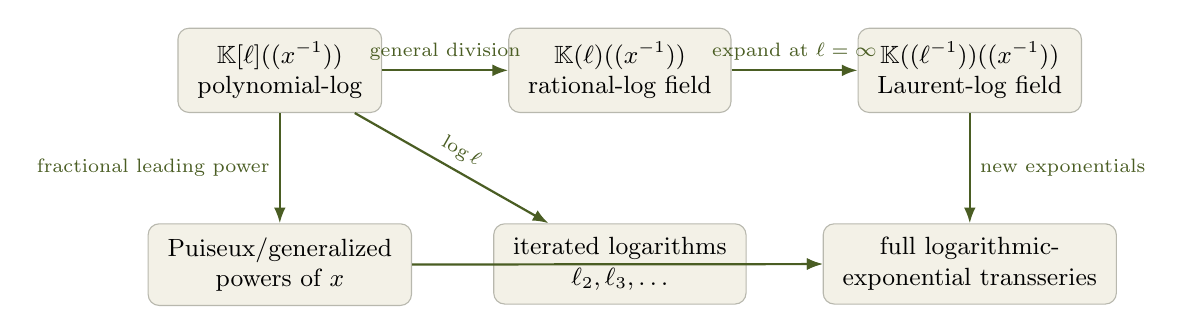
\begin{tikzpicture}[
  node distance=14mm and 16mm,
  box/.style={draw=rulegray,rounded corners,fill=shade,align=center,
              inner xsep=7pt,inner ysep=5pt,font=\small},
  arr/.style={-{Latex[length=2mm]},thick,color=accent}
]
\node[box] (pl) {\(\K[\ell]((x^{-1}))\)\\polynomial-log};
\node[box,right=of pl] (rl) {\(\K(\ell)((x^{-1}))\)\\rational-log field};
\node[box,right=of rl] (hl) {\(\K((\ell^{-1}))((x^{-1}))\)\\Laurent-log field};
\node[box,below=of pl] (pu) {Puiseux/generalized\\powers of \(x\)};
\node[box,below=of rl] (il) {iterated logarithms\\\(\ell_2,\ell_3,\ldots\)};
\node[box,below=of hl] (le) {full logarithmic-\\exponential transseries};
\draw[arr] (pl)--node[above,font=\scriptsize]{general division}(rl);
\draw[arr] (rl)--node[above,font=\scriptsize]{expand at \(\ell=\infty\)}(hl);
\draw[arr] (pl)--node[left,font=\scriptsize]{fractional leading power}(pu);
\draw[arr] (pl)--node[sloped,above,font=\scriptsize]{\(\log\ell\)}(il);
\draw[arr] (hl)--node[right,font=\scriptsize]{new exponentials}(le);
\draw[arr] (pu)--(le);
\draw[arr] (il)--(le);
\end{tikzpicture}
\end{center}

\subsection{A formal implicit-function principle}

Series reversal is one instance of a more general Newton--Hensel mechanism.
Let \(\Phi(x,y)\) be an expression built from PL coefficients and local analytic
operations in \(y\).  Suppose an approximation \(Y_0\in\PL\) satisfies
\[
  \Phi(x,Y_0)\in t^N{\PL}_{\ge0}
\]
and the partial derivative
\[
  \Phi_y(x,Y_0)=c+\FormalBigOAt{t}{t},
  \qquad c\in\K^\times,
\]
is a unit.  Then the Newton iteration
\begin{equation}\label{eq:implicit-Newton}
  Y_{j+1}=Y_j-\frac{\Phi(x,Y_j)}{\Phi_y(x,Y_j)}
\end{equation}
constructs a unique solution near \(Y_0\), with precision doubling under the
same Taylor estimates as in \cref{sec:reversion}.  The leading-unit condition is
the formal analogue of a nonzero Jacobian.

This principle covers algebraic equations, logarithmic implicit equations,
Riccati-type algebraic balances, and parameter-dependent inversions.  When
\(\Phi_y\) is not a unit, the correct response is usually not to force division,
but to refine the dominant balance and enlarge the monomial scale.

\section{Worked calculations}\label{sec:worked}

\subsection{Logarithm of a monomial-leading PL series}

Consider
\begin{equation}\label{eq:worked-log-F}
  F(x)=x^2\left(1+\ell t+(\ell^2-1)t^2\right).
\end{equation}
The leading coefficient after factoring \(x^2\) is the scalar \(1\), so the
logarithm stays in \(\PL\):
\[
  \log F=2\ell+\log(1+U),
  \qquad U=\ell t+(\ell^2-1)t^2.
\]
Expanding \(U-U^2/2+U^3/3-U^4/4+\cdots\) gives
\begin{align}
 \log F={}&2\ell+\ell t
 +\left(\frac{\ell^2}{2}-1\right)t^2
 +\left(-\frac{2\ell^3}{3}+\ell\right)t^3\nonumber\\
 &+\left(\frac{\ell^4}{4}-\frac12\right)t^4
 +\FormalBigOAt{t^5}{t}.
 \label{eq:worked-log-result}
\end{align}
Every coefficient at order \(t^N\) uses only powers \(U^r\) with \(r\le N\).

If the parenthesis in \eqref{eq:worked-log-F} were replaced by
\(\ell+1+\FormalBigOAt{t}{t}\), the logarithm would begin with \(\log\ell\) and leave the
one-log ring.  The difference is entirely in the leading coefficient.

\subsection{Triangular construction of \(\WrightOmega(x)\)}

Let \(f(y)=y+\log y\).  Starting with \(G_0=x\), compute the residual
\(R_j=f(G_j)-x\) and negate its leading coefficient as in
\eqref{eq:triangular-update}:
\begin{align*}
 G_0&=x,
 &R_0&=\ell,\\
 G_1&=x-\ell,
 &R_1&=-\ell t-\frac{\ell^2}{2}t^2-\frac{\ell^3}{3}t^3-\cdots,\\
 G_2&=x-\ell+\ell t,
 &R_2&=-\left(\frac{\ell^2}{2}-\ell\right)t^2
      +\left(-\frac{\ell^3}{3}+\ell^2\right)t^3+\cdots,\\
 G_3&=x-\ell+\ell t+
       \left(\frac{\ell^2}{2}-\ell\right)t^2,
 &R_3&=-\left(\frac{\ell^3}{3}-\frac{3\ell^2}{2}+\ell\right)t^3
      +\cdots.
\end{align*}
The next correction is therefore \(\LambertPolynomial{3}(\ell)t^3\).  In general, if
\[
  G_N=x+\sum_{n=0}^{N-1}\LambertPolynomial{n}(\ell)t^n,
\]
then
\begin{equation}\label{eq:Lambert-residual-staircase}
  f(G_N)-x=-\LambertPolynomial{N}(\ell)t^N+\FormalBigOAt{t^{N+1}}{t}.
\end{equation}
This identity offers another characterization of the Lambert polynomials and a
simple residual test for generated tables.

\subsection{Inverting \(y+a\log y+b/y+c/y^2\)}

Consider
\begin{equation}\label{eq:worked-abc-equation}
  x=y+a\log y+\frac{b}{y}+\frac{c}{y^2}.
\end{equation}
Set \(A(x)=a\ell+bt+ct^2\) in the Lagrange formula.  The inverse branch
asymptotic to \(x\) is
\begin{align}
 y={}&x-a\ell
 +\frac{a^2\ell-b}{x}\nonumber\\
 &+\frac{a^3(\ell^2-2\ell)-2ab\ell+2ab-2c}{2x^2}
 \nonumber\\
 &+\frac{1}{6x^3}\Bigl(
 2a^4\ell^3-9a^4\ell^2+6a^4\ell
 -6a^2b\ell^2+18a^2b\ell-6a^2b\nonumber\\
 &\hspace{31mm}-12ac\ell+6ac-6b^2\Bigr)
 +\FormalBigOAt{t^4}{t}.
 \label{eq:worked-abc-inverse}
\end{align}
Several structural checks are visible:
\begin{itemize}
\item the highest log power at level \(x^{-n}\) is supplied solely by the
  repeated logarithmic perturbation;
\item \(c\), which begins at \(x^{-2}\), first affects the inverse at the same
  level;
\item products such as \(b^2\) first occur when two rational perturbations can
  combine at a common level;
\item setting \(b=c=0\) leaves scaled Lambert polynomials.
\end{itemize}
Substitution of \eqref{eq:worked-abc-inverse} into
\eqref{eq:worked-abc-equation} cancels every term through \(x^{-3}\).

\subsection{A quotient followed by composition}

Let
\[
  Q(x)=\frac{1+\ell t}{1-\ell t+t^2}.
\]
Since the denominator is a unit, recurrence \eqref{eq:quotient-recurrence}
gives
\begin{equation}\label{eq:worked-Q}
  Q=1+2\ell t+(2\ell^2-1)t^2
    +(2\ell^3-3\ell)t^3
    +(2\ell^4-5\ell^2+1)t^4+\cdots.
\end{equation}
Now compose with \(G=x+\ell\).  The Taylor formula says
\[
  Q\circ G=Q+\ell Q'+\frac{\ell^2}{2}Q''+\cdots.
\]
To obtain terms through \(t^3\), only derivatives through order three can
contribute, and the derivative of a coefficient \(p_n(\ell)t^n\) is obtained by
\((\dlog-n)p_n\) at the next level.  The calculation is finite at every stage;
no direct expansion of a nested rational-log expression is required.

This example illustrates a useful workflow: normalize divisions first, cache
the resulting coefficient polynomials, then compose.  Reversing the order can
force larger intermediate expressions even though the final truncated answer is
the same.

\subsection{Power-log inversion versus branch-point inversion}

Compare two inverse problems.
\begin{align*}
  x&=y+\log y,\\
  x&=y^2+y.
\end{align*}
The first has derivative \(1+1/y\to1\) and belongs to the near-identity PL
group after dominant balance \(y\sim x\).  The second has dominant balance
\(y\sim x^{1/2}\), so the correct scale is Puiseux from the beginning:
\[
  y=\frac{-1+\sqrt{1+4x}}2
   =x^{1/2}-\frac12+\frac{1}{8}x^{-1/2}
    -\frac{1}{128}x^{-3/2}+\cdots.
\]
Trying an integer-power PL ansatz for the second equation cannot succeed.  A
dominant-balance analysis must precede coefficient recursion.

\subsection{A practical closure checklist}

Before performing a requested operation, ask:
\begin{enumerate}
\item What is the leading \(x\)-power, and is its exponent in the current
  exponent group?
\item Is the leading coefficient in \(\ell\) a unit of the coefficient ring?
\item Does a logarithm act on a scalar-leading unit, or will it create
  \(\log\ell\)?
\item For composition, does the inner argument tend to infinity with a
  controlled monomial leading term?
\item For reversal, is the leading derivative a unit?  If not, what ramified
  balance replaces the near-identity ansatz?
\item Which branch constants must be carried explicitly?
\item What output monomials are retained, and is that truncation region stable
  under all intermediate products?
\end{enumerate}
These questions turn most apparent ``transseries mysteries'' into routine
representation decisions.

\section{Conclusions and a compact structural picture}\label{sec:conclusion}

Polynomial-logarithmic transseries occupy a useful middle ground.  Ordinary
Laurent series are too small to survive the inversion of even the elementary
map \(y\mapsto y+\log y\), while the full logarithmic-exponential transseries
field contains much more structure than is needed for that problem.  The ring
\[
  \PL=\K[\ell]((t)),\qquad t=x^{-1},\quad \ell=\log x,
\]
is therefore not merely a pedagogical toy.  It is a sharply delimited
computational domain in which support, truncation, and coefficient arithmetic
are completely explicit.

The main conclusions of the preceding sections can be compressed as follows.

\begin{enumerate}
\item \textbf{Multiplication is unconditional.}
  Products are Cauchy convolutions over \(\K[\ell]\), and every requested
  coefficient is a finite sum.  The \(t\)-adic filtration makes truncated
  multiplication exact below the cutoff.

\item \textbf{Division is conditional.}
  A series is a unit of \(\K[\ell]((t))\) precisely when its leading
  coefficient is a nonzero scalar.  A nonconstant leading polynomial in
  \(\ell\) forces rational-log coefficients; an inverse power of \(\ell\)
  suggests Laurent-log or \(\ell^{-1}\)-adic coefficients instead.  This is a
  representation issue, not a failure of formal algebra.

\item \textbf{Differentiation and antidifferentiation are internal.}
  The identity
  \[
    D\bigl(t^n p(\ell)\bigr)
       =t^{n+1}(\partial_\ell-n)p(\ell)
  \]
  turns analytic differentiation into a shifted polynomial operator.  The
  corresponding first-order polynomial equations also give an antiderivative
  within the same class.

\item \textbf{Composition is an admissible partial operation.}
  Substitution becomes locally finite when the inner series has a controlled
  large leading monomial.  The most important case is the near-identity map
  \(G=x+H\), for which Taylor expansion is \(t\)-adically finite because every
  derivative raises the inverse-power level.  Arbitrary formal substitution is
  neither defined nor closed.

\item \textbf{Near-identity maps form a composition group.}
  Every \(F=x+A\), with \(A\) of nonnegative \(t\)-order, has a unique inverse
  of the same form.  Picard iteration proves existence, triangular matching
  exposes coefficient dependence, Newton iteration gives precision doubling,
  and Lagrange--B\"urmann gives the closed formula
  \[
    F^{\rev}=x+\sum_{r\ge1}\frac{(-1)^r}{r!}D^{r-1}(A^r).
  \]

\item \textbf{Dominant balance comes before algebra.}
  If the leading map behaves like \(cy^q\), then its inverse behaves like
  \(c^{-1/q}x^{1/q}\).  A nonintegral exponent requires a Puiseux-log scale;
  vanishing or singular leading derivatives may require a different scale
  again.  Reversion does not repair an incorrectly chosen monomial group.

\item \textbf{Lambert \(\LambertW\) is the canonical model.}
  Taking logarithms of \(we^w=z\) reduces every large branch to inversion of
  \(w+\log w\).  The resulting Lambert polynomials simultaneously encode the
  coefficient recurrence, the Lagrange differential formula, and the signed
  Stirling numbers of the first kind.
\end{enumerate}

\begin{summarybox}[The operational rule]
Normalize the dominant monomial first.  Then ask whether the leading
coefficient is a unit, whether every logarithm is applied to a scalar-leading
unit, and whether the inner argument of every composition is large in a
controlled way.  Once those three questions have affirmative answers,
coefficient extraction is finite and algorithmic.  If one answer is negative,
enlarge the scale before calculating.
\end{summarybox}

The distinction among formal existence, analytic asymptotic validity, and
convergence remains essential.  Formal PL algebra determines coefficients and
identities.  Analytic theorems justify substitution into actual functions and
control remainders.  Convergence, when available, is an additional property,
not part of the definition.  Keeping these layers separate is what makes the
small calculus reliable and extensible.

\appendix

\section{Coefficient extraction in closed form}\label{app:coefficients}

This appendix records formulas useful for direct implementations and for
checking hand calculations.  They contain no infinite sums at a fixed output
level.

\subsection{Finite convolution polynomials}

Let
\[
  H=\sum_{j\ge0}h_j(\ell)t^j.
\]
For integers \(m,r\ge0\), define
\begin{equation}\label{eq:Cmr-definition}
  C_{m,r}(h_0,h_1,\ldots)
  =\sum_{\substack{j_1,\ldots,j_r\ge0\\j_1+\cdots+j_r=m}}
      h_{j_1}\cdots h_{j_r},
\end{equation}
with \(C_{0,0}=1\) and \(C_{m,0}=0\) for \(m>0\).  Equivalently,
\[
  H^r=\sum_{m\ge0}C_{m,r}t^m.
\]
The recurrence
\begin{equation}\label{eq:Cmr-recurrence}
  C_{m,r+1}=\sum_{j=0}^{m}h_j C_{m-j,r}
\end{equation}
computes all values in a triangular table.  If \(h_0=0\), then
\(C_{m,r}=0\) for \(m<r\), and these are the ordinary partial convolution
polynomials underlying ordinary Bell polynomials.

\subsection{A coefficient formula for near-identity composition}

For \(n\in\IntegerNumbers\) and \(r\ge0\), set
\begin{equation}\label{eq:Delta-nr-app}
  \Delta_{n,r}
  =\prod_{q=0}^{r-1}(\partial_\ell-n-q),
  \qquad \Delta_{n,0}=1.
\end{equation}
Let
\[
  F=\sum_{n\ge n_0}f_n(\ell)t^n,
  \qquad G=x+H,
  \qquad H=\sum_{j\ge0}h_j(\ell)t^j.
\]
Then \(F\circ G=\sum_N c_N(\ell)t^N\), where
\begin{equation}\label{eq:composition-coefficient-Cmr}
\boxed{
  c_N=
  \sum_{n=n_0}^{N}\;
  \sum_{r=0}^{N-n}
    \frac{C_{N-n-r,r}}{r!}\,
    \Delta_{n,r}f_n.
}
\end{equation}
All polynomial arguments \(h_0,h_1,\ldots\) in \(C_{m,r}\) are suppressed in
\eqref{eq:composition-coefficient-Cmr}.

\begin{proof}
Taylor's formula and the repeated-derivative identity give
\[
  F(x+H)
  =\sum_{r\ge0}\frac{H^r}{r!}D^rF
  =\sum_{r\ge0}\sum_{m\ge0}\sum_{n\ge n_0}
     \frac{C_{m,r}}{r!}\,
     \Delta_{n,r}f_n\,t^{m+n+r}.
\]
The coefficient of \(t^N\) has \(m=N-n-r\), which yields
\eqref{eq:composition-coefficient-Cmr}.  The inequalities \(m\ge0\) and
\(r\ge0\) make both displayed sums finite.
\end{proof}

Two special cases are especially useful.  If \(H=h_0(\ell)\) has no positive
\(t\)-levels, then only \(m=0\) occurs and
\begin{equation}\label{eq:composition-pure-log-shift}
  c_N=\sum_{n=n_0}^{N}
    \frac{h_0^{N-n}}{(N-n)!}\,
    \Delta_{n,N-n}f_n.
\end{equation}
Thus composition by \(x+\ell\), \(x+a\ell+b\), or any polynomial-logarithmic
shift at level zero has a single-sum coefficient formula.  If instead
\(h_0=0\), then the extra vanishing \(C_{m,r}=0\) for \(m<r\) sharply reduces
the summation region.

\subsection{Fa\`a di Bruno inside the PL ring}

Let \(\Phi\) be analytic at the scalar leading value of \(F\), so that
\(\Phi(F)\) is defined by the local functional calculus of
\cref{subsec:field-extensions}.  For \(m\ge1\), the usual Fa\`a di Bruno
identity remains valid:
\begin{equation}\label{eq:faa-di-bruno-PL}
  D^m\Phi(F)
   =\sum_{k=1}^{m}\Phi^{(k)}(F)
      B_{m,k}\bigl(F',F'',\ldots,F^{(m-k+1)}\bigr),
\end{equation}
where the exponential partial Bell polynomial is
\begin{equation}\label{eq:exponential-Bell-definition}
 B_{m,k}(z_1,z_2,\ldots)
 =\sum
   \frac{m!}{j_1!j_2!\cdots}
   \prod_{r\ge1}\left(\frac{z_r}{r!}\right)^{j_r}.
\end{equation}
The sum ranges over \(\sum j_r=k\) and \(\sum rj_r=m\).  It is finite before
any transseries substitution is made.  Since differentiation, multiplication,
and the relevant local analytic functions are all defined in the PL ring, the
classical formal proof applies verbatim.

Formula \eqref{eq:faa-di-bruno-PL} is useful in two places.  First, it expands
high Taylor derivatives occurring in composition.  Second, it expresses the
Lagrange terms \(D^{r-1}(A^r)\) as differential polynomials in \(A\), making
universal inverse formulas independent of any chosen coefficient basis.

\subsection{Fast recurrences for elementary local functions}

The following recurrences use an \emph{auxiliary} derivation
\(\partial_t\) that holds \(\ell\) fixed.  It is legitimate for coefficient
extraction in the abstract power-series ring \(\K[\ell][[t]]\), but it is not
the analytic derivative with respect to \(t\), because analytically
\(\ell=-\log t\).

Let \(U=\sum_{n\ge1}u_nt^n\).

For \(E=\exp U=\sum_{n\ge0}e_nt^n\),
\begin{equation}\label{eq:exp-coefficient-recurrence}
  e_0=1,
  \qquad
  ne_n=\sum_{j=1}^{n}j u_j e_{n-j}.
\end{equation}
This follows from \(\partial_tE=E\partial_tU\).

For \(L=\log(1+U)=\sum_{n\ge1}\lambda_nt^n\),
\begin{equation}\label{eq:log-coefficient-recurrence}
  \lambda_n=u_n-\frac1n
  \sum_{j=1}^{n-1}(n-j)u_j\lambda_{n-j}.
\end{equation}
Indeed, \((1+U)\partial_tL=\partial_tU\).

For \(P=(1+U)^\alpha=\sum_{n\ge0}p_nt^n\),
\begin{equation}\label{eq:power-coefficient-recurrence}
  p_0=1,
  \qquad
  np_n=\alpha n u_n+
   \sum_{j=1}^{n-1}\bigl(\alpha j-(n-j)\bigr)u_jp_{n-j}.
\end{equation}
This comes from \((1+U)\partial_tP=\alpha P\partial_tU\).  The formulas are
valid over any characteristic-zero coefficient algebra, hence in particular
over \(\K[\ell]\), \(\K(\ell)\), or a Puiseux-log coefficient ring.

\section{Further details on reversal}\label{app:reversal}

\subsection{Universal terms through the fifth Lagrange index}

Grouping the inverse by Lagrange index rather than by \(t\)-level gives
\begin{align}
 F^{\rev}={}&x-A
 +AA'\nonumber\\
 &-A(A')^2-\frac12A^2A''\nonumber\\
 &+A(A')^3+\frac32A^2A'A''+\frac16A^3A'''\nonumber\\
 &-A(A')^4-3A^2(A')^2A''-\frac12A^3(A'')^2
   -\frac23A^3A'A'''-\frac1{24}A^4A''''
 +\cdots.\label{eq:inverse-universal-through-five}
\end{align}
The first line after \(x-A\) is the \(r=2\) Lagrange term, the next is
\(r=3\), and so on.  For example,
\[
 \frac{1}{24}D^3(A^4)
 =A(A')^3+\frac32A^2A'A''+\frac16A^3A''',
\]
while
\begin{align*}
 -\frac1{120}D^4(A^5)={}&-A(A')^4-3A^2(A')^2A''
 -\frac12A^3(A'')^2\\
 &-\frac23A^3A'A'''-\frac1{24}A^4A''''.
\end{align*}
These formulas are excellent for low-order symbolic work, but at high order the
compact derivative form should be retained to avoid expression swell.

\subsection{A substitution certificate for a truncated inverse}

\begin{proposition}[Finite certificate]\label{prop:inverse-certificate}
Let \(F=x+A\) with \(A\in{\PL}_{\ge0}\), and let
\[
  G_N=x+\sum_{j=0}^{N}b_j(\ell)t^j.
\]
Then \(G_N\) is the truncation through level \(N\) of \(F^{\rev}\) if and only
if
\begin{equation}\label{eq:inverse-certificate}
  F\circ G_N-x\in t^{N+1}\K[\ell][[t]].
\end{equation}
The equivalent left certificate is
\(G_N\circ F-x\in t^{N+1}\K[\ell][[t]]\).
\end{proposition}

\begin{proof}
Necessity follows by truncating the exact identity.  Conversely, let \(G\) be
the unique inverse supplied by the near-identity group theorem.  If \(G_N-G\)
had first nonzero term \(q(\ell)t^m\) with \(m\le N\), then Taylor expansion of
\(F\) at \(G\) would give
\[
  F\circ G_N-F\circ G
  =(F'\circ G)q(\ell)t^m+\FormalBigOAt{t^{m+1}}{t}.
\]
Because \(F'\circ G=1+\FormalBigOAt{t}{t}\), the coefficient at level \(m\) would be
\(q\ne0\), contradicting \eqref{eq:inverse-certificate}.  Hence
\(G_N-G\in t^{N+1}{\PL}_{\ge0}\).
\end{proof}

This proposition is the simplest robust test for software.  It avoids comparing
the output with a second implementation term by term: compose once, truncate,
and require an exact zero polynomial at every retained level.

\subsection{Ramified reversal after dominant balance}

Near-identity reversal is only one normal form.  Suppose more generally that
\begin{equation}\label{eq:ramified-leading-map}
  F(y)=c y^q\bigl(1+U(y)\bigr),
  \qquad c\ne0,
  \qquad U(y)\prec1,
\end{equation}
where \(q\in\RationalNumbers_{>0}\).  Choose a branch of
\(d=c^{-1/q}\) and write
\begin{equation}\label{eq:ramified-inverse-ansatz}
  y=d x^{1/q}(1+V).
\end{equation}
Substitution into \eqref{eq:ramified-leading-map} gives
\begin{equation}\label{eq:ramified-normalized-equation}
  (1+V)^q
  \bigl(1+U(d x^{1/q}(1+V))\bigr)=1.
\end{equation}
The derivative of the left side with respect to \(V\) has scalar leading value
\(q\), so the formal implicit-function recursion is triangular.  The correct
ambient ring is generated by \(x^{-1/q}\) and the logarithms created by
composition.  Thus a branch point does not destroy reversibility; it changes
the exponent group and makes branch selection part of the leading data.

For \(q=1\), this normalization reduces to the monomial-leading composition
calculus.  For \(q=2\), it explains the half-integer expansion of the inverse of
\(y^2+y\).  If \(q\) is irrational, a Hahn group containing \(q^{-1}\IntegerNumbers\) is
required rather than an ordinary Puiseux group.

\subsection{Direct implicit recursion}

Consider an equation
\begin{equation}\label{eq:implicit-Psi-equation}
  \Psi(x,Y)=0,
  \qquad
  Y=Y_0+\sum_{n\ge1}y_n(\ell)t^n,
\end{equation}
where all operations in \(\Psi\) are admissible and
\(\partial_Y\Psi(x,Y_0)\) has a nonzero scalar leading coefficient.  Suppose
\(y_1,\ldots,y_{N-1}\) have already been determined.  Inserting
\(Y_{<N}+q(\ell)t^N\) changes the residual at its first undecided level by
\begin{equation}\label{eq:implicit-linearization-level}
  \bigl(\partial_Y\Psi(x,Y_0)\bigr)_{\mathrm{lead}}
  q(\ell)t^N.
\end{equation}
All nonlinear occurrences of \(q t^N\) are of higher level.  Therefore the
level-\(N\) equation is linear in \(q\), and division by the scalar leading
coefficient determines it uniquely.  This is the coefficient-level content of
the filtered implicit-function principle and explains why triangular matching
works far beyond literal compositional inverses.

\section{Lambert-polynomial identities and checks}\label{app:lambert}

\subsection{Coefficient triangle}

Write
\begin{equation}\label{eq:Lambert-coefficient-triangle}
  \LambertPolynomial{n}(X)=\sum_{m=1}^{n}\lambda_{n,m}X^m,
  \qquad n\ge1.
\end{equation}
The integral recurrence gives
\begin{equation}\label{eq:lambda-triangle-recurrence}
  \lambda_{n+1,m}
   =-\lambda_{n,m}+\frac{n}{m}\lambda_{n,m-1},
\end{equation}
where \(\lambda_{n,0}=0\).  The boundary data are
\begin{equation}\label{eq:lambda-boundary}
  \lambda_{n,1}=(-1)^{n+1},
  \qquad
  \lambda_{n,n}=\frac1n.
\end{equation}
Equivalently,
\begin{equation}\label{eq:lambda-Stirling}
  \lambda_{n,m}
   =\frac{(-1)^{n+1}}{m!}
      s(n,n-m+1).
\end{equation}
Thus the entire table can be generated using only exact integer arithmetic
followed by division by \(m!\).

\subsection{A differential identity}

Differentiating the generating equation
\[
  \log(1+T\mathcal L)+\mathcal L=-X
\]
with respect to \(X\) gives
\begin{equation}\label{eq:Lambert-generating-X-derivative}
  \partial_X\mathcal L
  =-\frac{1+T\mathcal L}{1+T+T\mathcal L}.
\end{equation}
Together with the \(T\)-equation
\[
  T\mathcal L\,\partial_T\mathcal L
  +(1+T)\partial_T\mathcal L+\mathcal L=0,
\]
this gives independent recurrences for derivatives and coefficients.  In a
computer algebra system, checking both partial differential identities is a
stronger test than checking the first few expanded polynomials.

At the level of \(\WrightOmega\), implicit differentiation of
\(\WrightOmega+\log\WrightOmega=x\) yields
\begin{equation}\label{eq:omega-derivative-app}
  \WrightOmega'(x)=\frac{\WrightOmega(x)}{1+\WrightOmega(x)}.
\end{equation}
Substitution of \(\WrightOmega=x+\sum \LambertPolynomial{n}(\ell)x^{-n}\) into
\eqref{eq:omega-derivative-app} reproduces the Lambert recurrence after
coefficient collection.  Hence the inverse equation, the differential equation,
and the Stirling formula are three mutually independent certificates for the
same polynomial family.

\subsection{Scaling law}

The inverse of
\begin{equation}\label{eq:scaled-Lambert-map}
  y+a\log y=x,
  \qquad a\ne0,
\end{equation}
can be reduced exactly to Wright omega.  Put \(y=a u\); then
\[
  u+\log u=\frac{x}{a}-\log a,
\]
with a consistent logarithm of \(a\).  Consequently,
\begin{equation}\label{eq:scaled-omega-exact}
  y=a\,\WrightOmega\!\left(\frac{x}{a}-\log a\right).
\end{equation}
Expanding the right side in the original variable \(x\) recovers the powers
\(a^{n+1}\LambertPolynomial{n}(\log x)\) at their highest logarithmic degree, together with the
lower-degree corrections caused by the shift \(-\log a\) and by re-expanding
\(\log(x/a-a\log a)\).  This identity is a useful exact benchmark for generic
reversion code with symbolic parameters.

\subsection{Why one should retain the nested variables}

For direct evaluation of \(\LambertW_k(z)\), it is usually preferable to retain
\[
  \xi_k=\PrincipalLogarithm z+2\pi \ImaginaryUnit k,
  \qquad \eta_k=\log\xi_k,
\]
and evaluate
\[
  \LambertW_k(z)\approx \xi_k+\sum_{n=0}^{N}\frac{\LambertPolynomial{n}(\eta_k)}{\xi_k^n}
\]
rather than fully expand in powers of \((\PrincipalLogarithm z)^{-1}\) and \(2\pi \ImaginaryUnit k\).
The nested form preserves branch information, has smaller intermediate
expressions, and permits Horner evaluation of each \(\LambertPolynomial{n}\).  A further
re-expansion should be performed only when a downstream calculation requires a
single prescribed monomial scale.

\section{Notation and operation tables}\label{app:tables}

\subsection{Core notation}

\begin{longtable}{@{}p{0.23\textwidth}p{0.69\textwidth}@{}}
\caption{Notation used throughout the article.}\label{tab:notation}\\
\toprule
Symbol & Meaning\\
\midrule
\endfirsthead
\toprule
Symbol & Meaning\\
\midrule
\endhead
\(t=x^{-1}\) & small inverse-power variable as \(x\to\infty\)\\
\(\ell=\log x\) & first logarithmic scale\\
\(\PL=\K[\ell]((t))\) & polynomial-logarithmic Laurent-series ring\\
\(\ordx F\) & least exponent of \(t\) occurring in \(F\)\\
\(\degell p\) & degree of a coefficient polynomial in \(\ell\)\\
\(\Delta_{n,r}\) & \(\prod_{q=0}^{r-1}(\partial_\ell-n-q)\), the shifted derivative operator\\
\(F^{\rev}\) & compositional inverse of \(F\), not multiplicative reciprocal\\
\(\LambertPolynomial{n}(X)\) & Lambert polynomial at inverse-power level \(n\)\\
\(s(n,k)\) & signed Stirling number of the first kind\\
\(\UnsignedStirlingFirstKind{n}{k}\) & unsigned Stirling cycle number\\
\(\as\) & Poincar\'e asymptotic expansion in the stated scale\\
\(\BigOAt{x^{-N}(\log x)^d}{x\to+\infty}\) & analytic remainder bound on the stated limiting domain\\
\bottomrule
\end{longtable}

\subsection{Closure table}

\begin{longtable}{@{}p{0.22\textwidth}p{0.25\textwidth}p{0.45\textwidth}@{}}
\caption{Closure of the basic PL class and the usual repair when closure fails.}\label{tab:closure-summary}\\
\toprule
Operation & Closed in \(\K[\ell]((t))\)? & Condition or minimal enlargement\\
\midrule
\endfirsthead
\toprule
Operation & Closed in \(\K[\ell]((t))\)? & Condition or minimal enlargement\\
\midrule
\endhead
Addition, subtraction & yes & no qualification\\
Multiplication & yes & Cauchy convolution over \(\K[\ell]\)\\
Differentiation & yes & \(D(t^np)=t^{n+1}(\partial_\ell-n)p\)\\
Antidifferentiation & yes & solve a first-order polynomial equation at each level\\
Reciprocal & only for units & scalar leading coefficient; otherwise use \(\K(\ell)((t))\) or a Laurent-log scale\\
Integer powers & yes for units and finite nonnegative powers & negative powers require a unit\\
Rational powers & conditionally & scalar-leading unit after extracting a monomial; use Puiseux exponents if needed\\
Logarithm & conditionally & extract \(c x^q\); a leading \(\ell^d\) creates \(\log\ell\)\\
Exponential & rarely & allowed for infinitesimal arguments; a nonzero polynomial in \(\ell\) may change the monomial group\\
Composition & conditionally & inner series must be large with controlled monomial leading term\\
Near-identity reversal & yes & \(F=x+A\), \(\ordx A\ge0\)\\
General reversal & conditionally & determine dominant balance; often Puiseux-log or Hahn enlargement\\
\bottomrule
\end{longtable}

\subsection{A minimal implementation checklist}

A reliable finite-precision implementation should enforce the following
invariants.

\begin{enumerate}
\item Store each coefficient in canonical polynomial form and omit exact zero
  levels.
\item Attach the exponent group and coefficient domain to every series value;
  never silently coerce \(\K[\ell]\) to \(\K(\ell)\) or \(\IntegerNumbers\) exponents to
  \(\RationalNumbers\) exponents.
\item Normalize a nonzero series into leading monomial, leading coefficient,
  and scalar-leading unit before applying reciprocal, logarithm, or a rational
  power.
\item Propagate a target truncation through every product, derivative, and
  composition.  Do not form terms that provably lie beyond the target.
\item Carry logarithm branches and fractional-power roots as explicit metadata
  in complex calculations.
\item Verify division by multiplying back, verify composition with an
  independently truncated direct substitution, and verify reversal using
  \cref{prop:inverse-certificate}.
\item For numerical use, estimate terms at the actual argument and truncate
  near the smallest term unless a convergence theorem applies.
\end{enumerate}

\clearpage
\begin{thebibliography}{99}

\bibitem{ADHTransseries}
M. Aschenbrenner, L. van den Dries, and J. van der Hoeven,
\emph{Asymptotic Differential Algebra and Model Theory of Transseries},
Annals of Mathematics Studies, vol.~195, Princeton University Press,
Princeton, 2017.

\bibitem{CohenLambert}
H. Cohen,
``Lambert \(\LambertW\)-Function Branch Identities,''
\emph{arXiv preprint} arXiv:2012.11698, revised 2021.

\bibitem{Corless1996}
R. M. Corless, G. H. Gonnet, D. E. G. Hare, D. J. Jeffrey, and D. E. Knuth,
``On the Lambert \(\LambertW\) Function,''
\emph{Advances in Computational Mathematics} \textbf{5} (1996), 329--359,
\href{https://doi.org/10.1007/BF02124750}{doi:10.1007/BF02124750}.

\bibitem{DLMFLambert}
NIST Digital Library of Mathematical Functions,
``\S4.13 Lambert \(\LambertW\)-Function,'' in \emph{DLMF}, version 1.2.7,
release date June 15, 2026,
\url{https://dlmf.nist.gov/4.13}.

\bibitem{EdgarBeginners}
G. A. Edgar,
``Transseries for Beginners,''
\emph{Real Analysis Exchange} \textbf{35} (2009/2010), no.~2, 253--310,
\href{https://doi.org/10.14321/realanalexch.35.2.0253}{doi:10.14321/realanalexch.35.2.0253};
also arXiv:0801.4877.

\bibitem{EdgarComposition}
G. A. Edgar,
``Transseries: Composition, Recursion, and Convergence,''
\emph{arXiv preprint} arXiv:0909.1259, 2009.

\bibitem{GesselLagrange}
I. M. Gessel,
``Lagrange Inversion,''
\emph{arXiv preprint} arXiv:1609.05988, 2016.

\bibitem{Hahn1907}
H. Hahn,
``\"Uber die nichtarchimedischen Gr\"o\ss ensysteme,''
\emph{Sitzungsberichte der Kaiserlichen Akademie der Wissenschaften Wien,
Mathematisch-Naturwissenschaftliche Klasse} \textbf{116} (1907), 601--655.

\bibitem{SalvyShackell1992}
B. Salvy and J. R. Shackell,
``Asymptotic Expansions of Functional Inverses,''
in P. S. Wang (ed.), \emph{Symbolic and Algebraic Computation: ISSAC '92},
ACM Press, New York, 1992, pp.~130--137,
\href{https://doi.org/10.1145/143242.143292}{doi:10.1145/143242.143292}.

\bibitem{VanDerHoeven2006}
J. van der Hoeven,
\emph{Transseries and Real Differential Algebra},
Lecture Notes in Mathematics, vol.~1888, Springer, Berlin, 2006,
\href{https://doi.org/10.1007/3-540-35590-1}{doi:10.1007/3-540-35590-1}.

\end{thebibliography}

\end{document}
